\chapter{Results}

We evaluate our tool by describing a number of real world cases where we were able to use our tool.
Firstly we reproduce the issue underlying the work of \mono{inspection-testing} \cite{inspection_testing}, which
also serves as a comprehensive, didactic example of how to use our tool.
The second case study is about stream fusion and focuses on the way that the theory differs from the true implementation.
In doing so, it covers a large spectrum of the optimisation pipeline.
Thirdly, we present how we were able to use our tool to find a performance bug in GHC itself and how we were furthermore
able to use it to evaluate a possible solution.
Finally, we compare our experience with the tool with that of using the existing output that can
be obtained from GHC today.

\section{Diagnosing a failing inspection test in \mono{Text}}

Hearkening back to \mono{inspection-testing} discussed in \cref{section:introduction_inspection_testing}, we put
ourselves in the shoes of a programmer who gets surprised by a failing inspection test and reason how we might
employ HsComprehension to diagnose the problem. 

To summarize, we expected that the function \mono{countChars} -- which counts the number of characters in a \mono{ByteString}
by composing three functions in the \mono{Text} library -- will in its final form not actually construct a \mono{Text} value.

\paragraph{1. Isolate the problem}
Modules typically contain more than 1 function and during the core2core transformations many more auxiliary functions are
added. Furthermore, many functions are inlined to produce ever more code. Despite the tool being designed with features to 
comprehend medium-sized modules, it is still most helpful to temporarily isolate the failing test case into a separate module:

\begin{minted}{haskell}
{-# LANGUAGE TemplateHaskell #-}

module InspectionTests where

import Test.Inspection
import qualified Data.Text as T
import qualified Data.Text.Encoding as TE
import Data.ByteString

countChars :: ByteString -> Int
countChars = T.length . T.toUpper . TE.decodeUtf8

-- the failing test case
inspect $ 'countChars `hasNoType` ''T.Text
\end{minted}

The following error is produced by the build:

\begin{minted}{sh}
app/InspectionTests.hs:21:1: countChars `hasNoType` Data.Text.Internal.Text failed:
# ...
# 700 lines of Core as seen at the end of the core2core pipeline
# ...
\end{minted}

700 lines of textual data is generated by \mono{inspection-testing} from just this one function!
It is also incomplete in the sense that it does not show the process that produced this final
artifact.

\paragraph{2. Creating a capture}

Because we only want to create a capture of this module, we can use an exported TemplateHaskell primitive
that registers the plugin for the current module only by simply adding the \mono{dumpThisModule} snippet 
anywhere at the top level: 

\begin{listing}[H]
\begin{minted}{haskell}
{-# LANGUAGE TemplateHaskell #-}
import HsComprehension.Plugin (dumpThisModule)

...

dumpThisModule
\end{minted}
\end{listing}

Following a successful build, we can bundle the generated artifacts to a zip archive by running:

\begin{listing}[H]
\begin{minted}{sh}
$ cabal run hs-comprehension-zip
Attempting to archive dump files in ./dist-newstyle/coredump-Default
Archiving 23 files
Created /home/hugo/repos/hs-comprehension/test-project/dist-newstyle/Default.zip
\end{minted}
\end{listing}

\paragraph{3. Finding the root cause}
We navigate to \href{https://core.hugopeters.me}{core.hugopeters.me} and upload the zip archive we just
produced.

\begin{figure}[H]
\centering
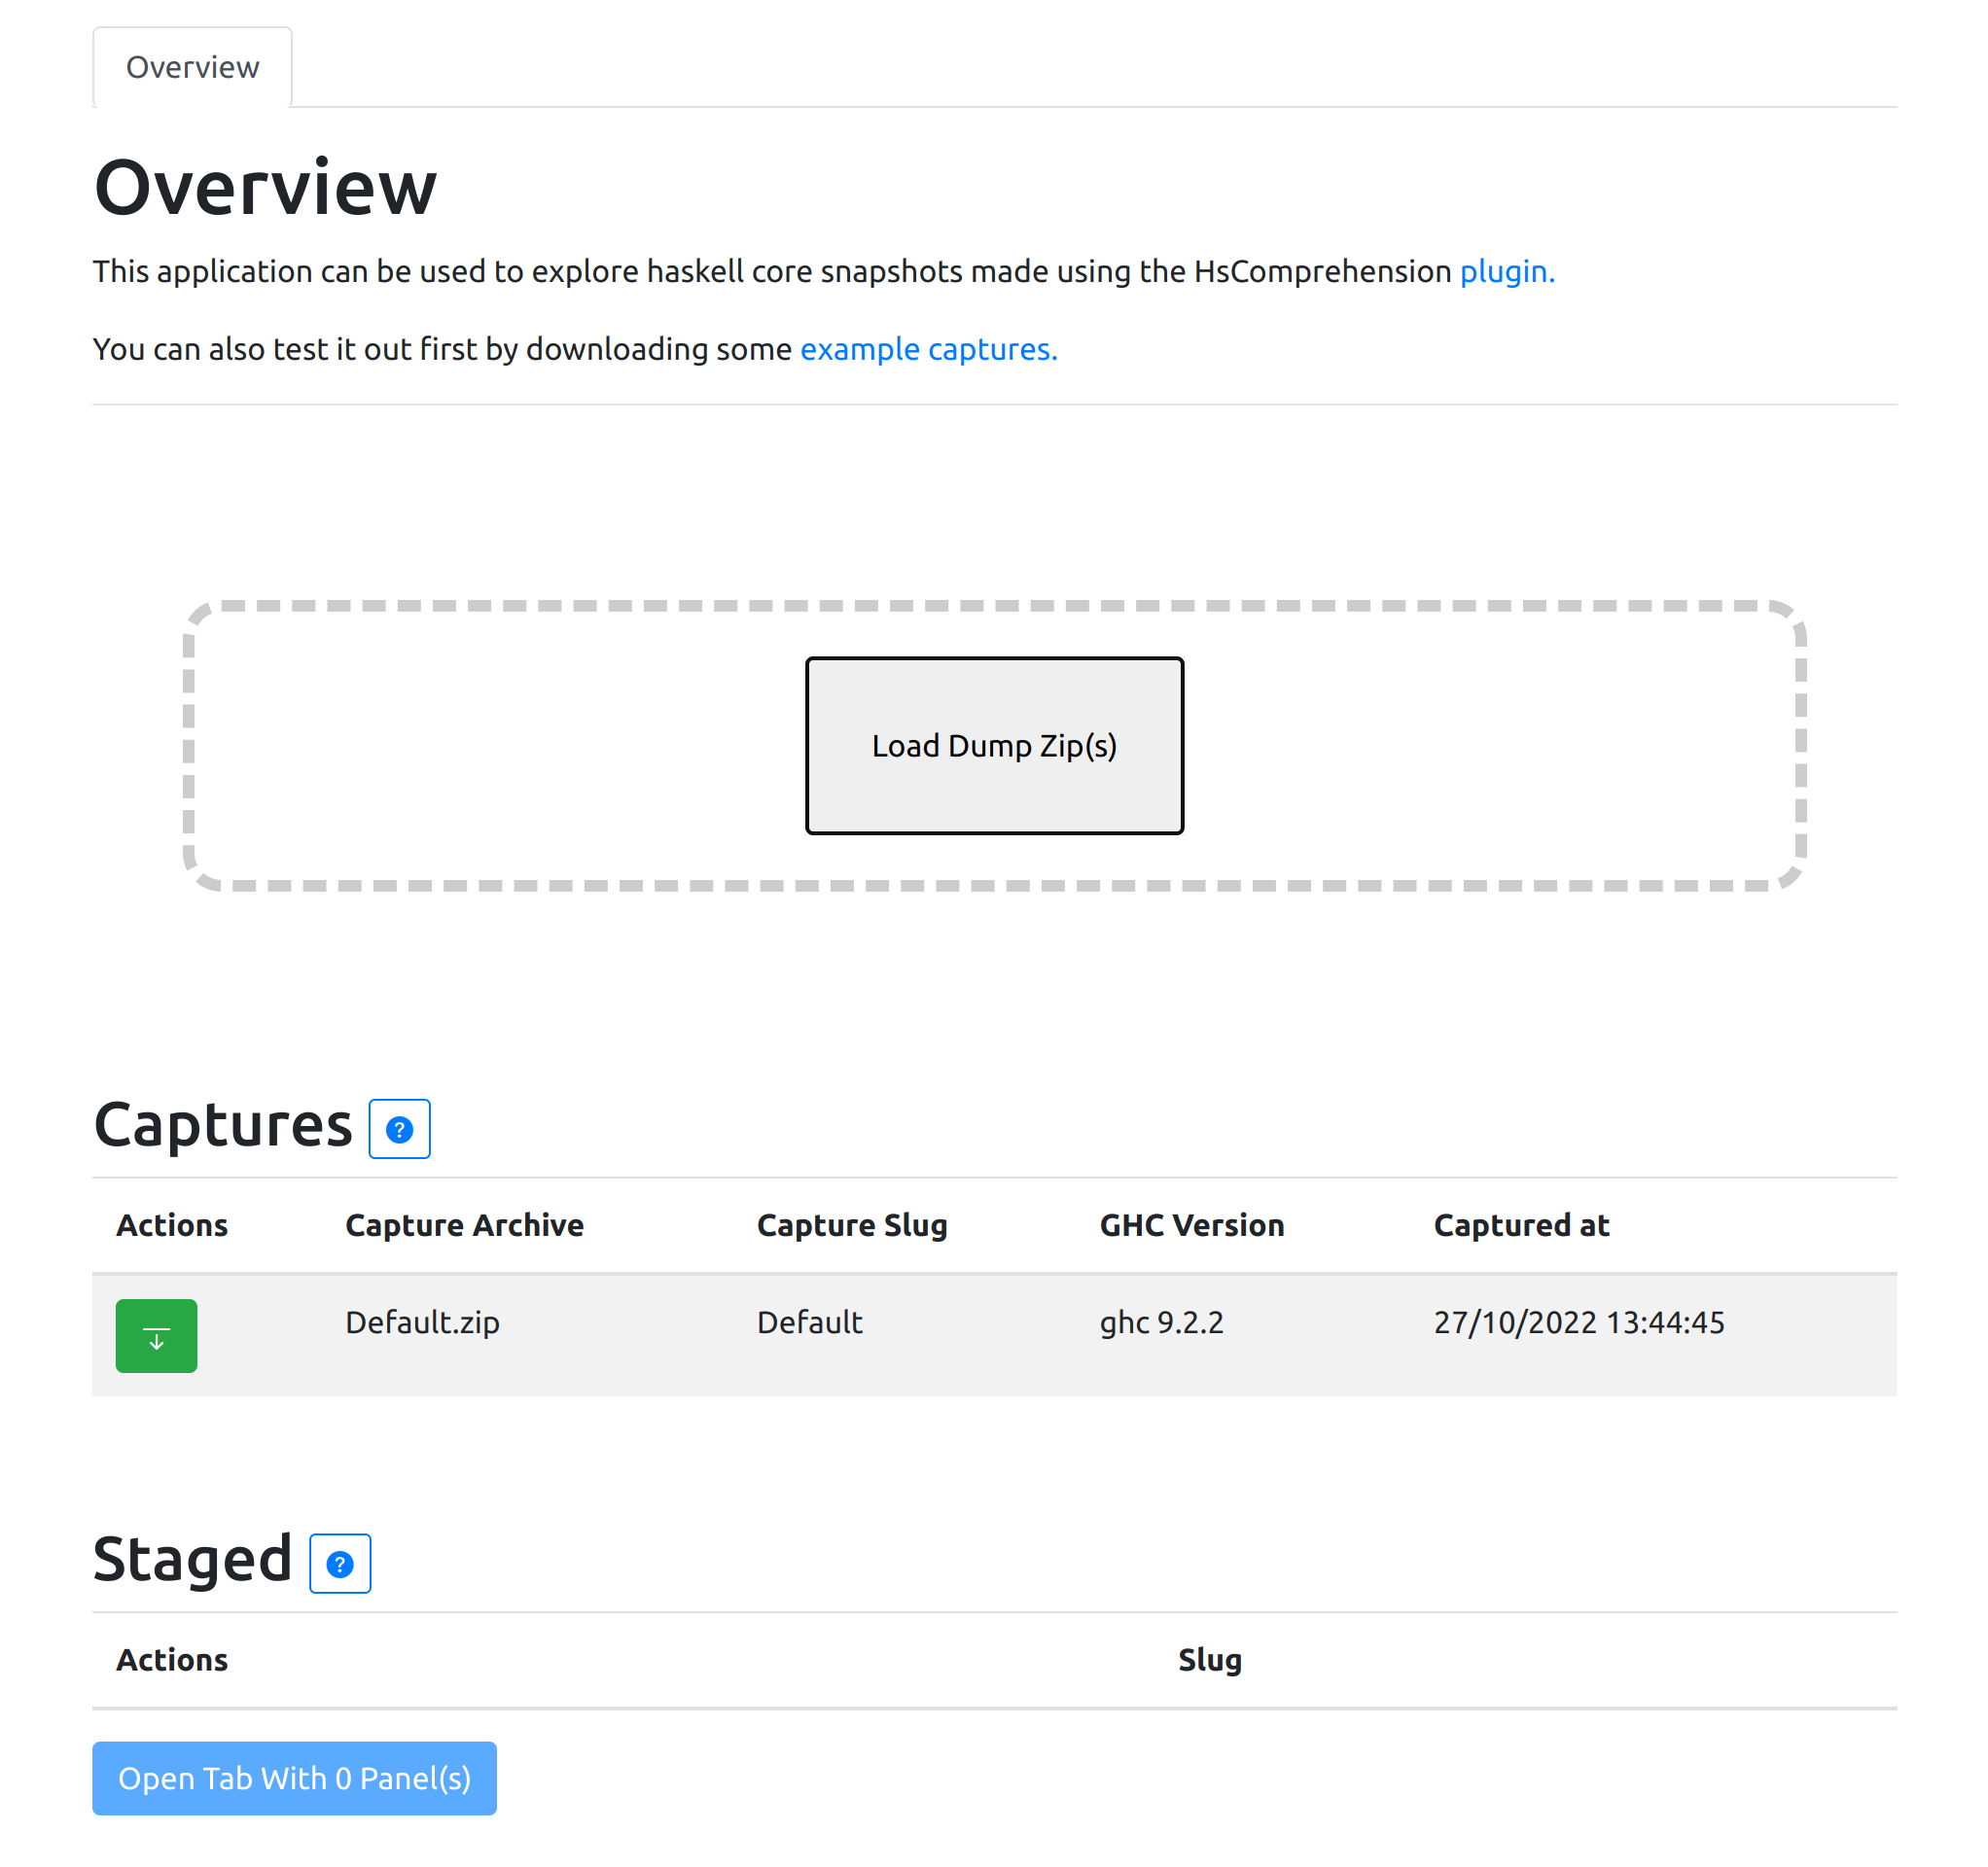
\includegraphics[width=0.8\textwidth]{figs/countchars_1.png}
\label{fig:countchars_1}
\end{figure}

We then click the green arrow to reference the capture in the staging area. Here we could elect to stage more
than one capture if we want to compare them. In this case we are only interested in the current situation, and so we
just open a single panel tab with this single capture


\begin{figure}[H]
\centering
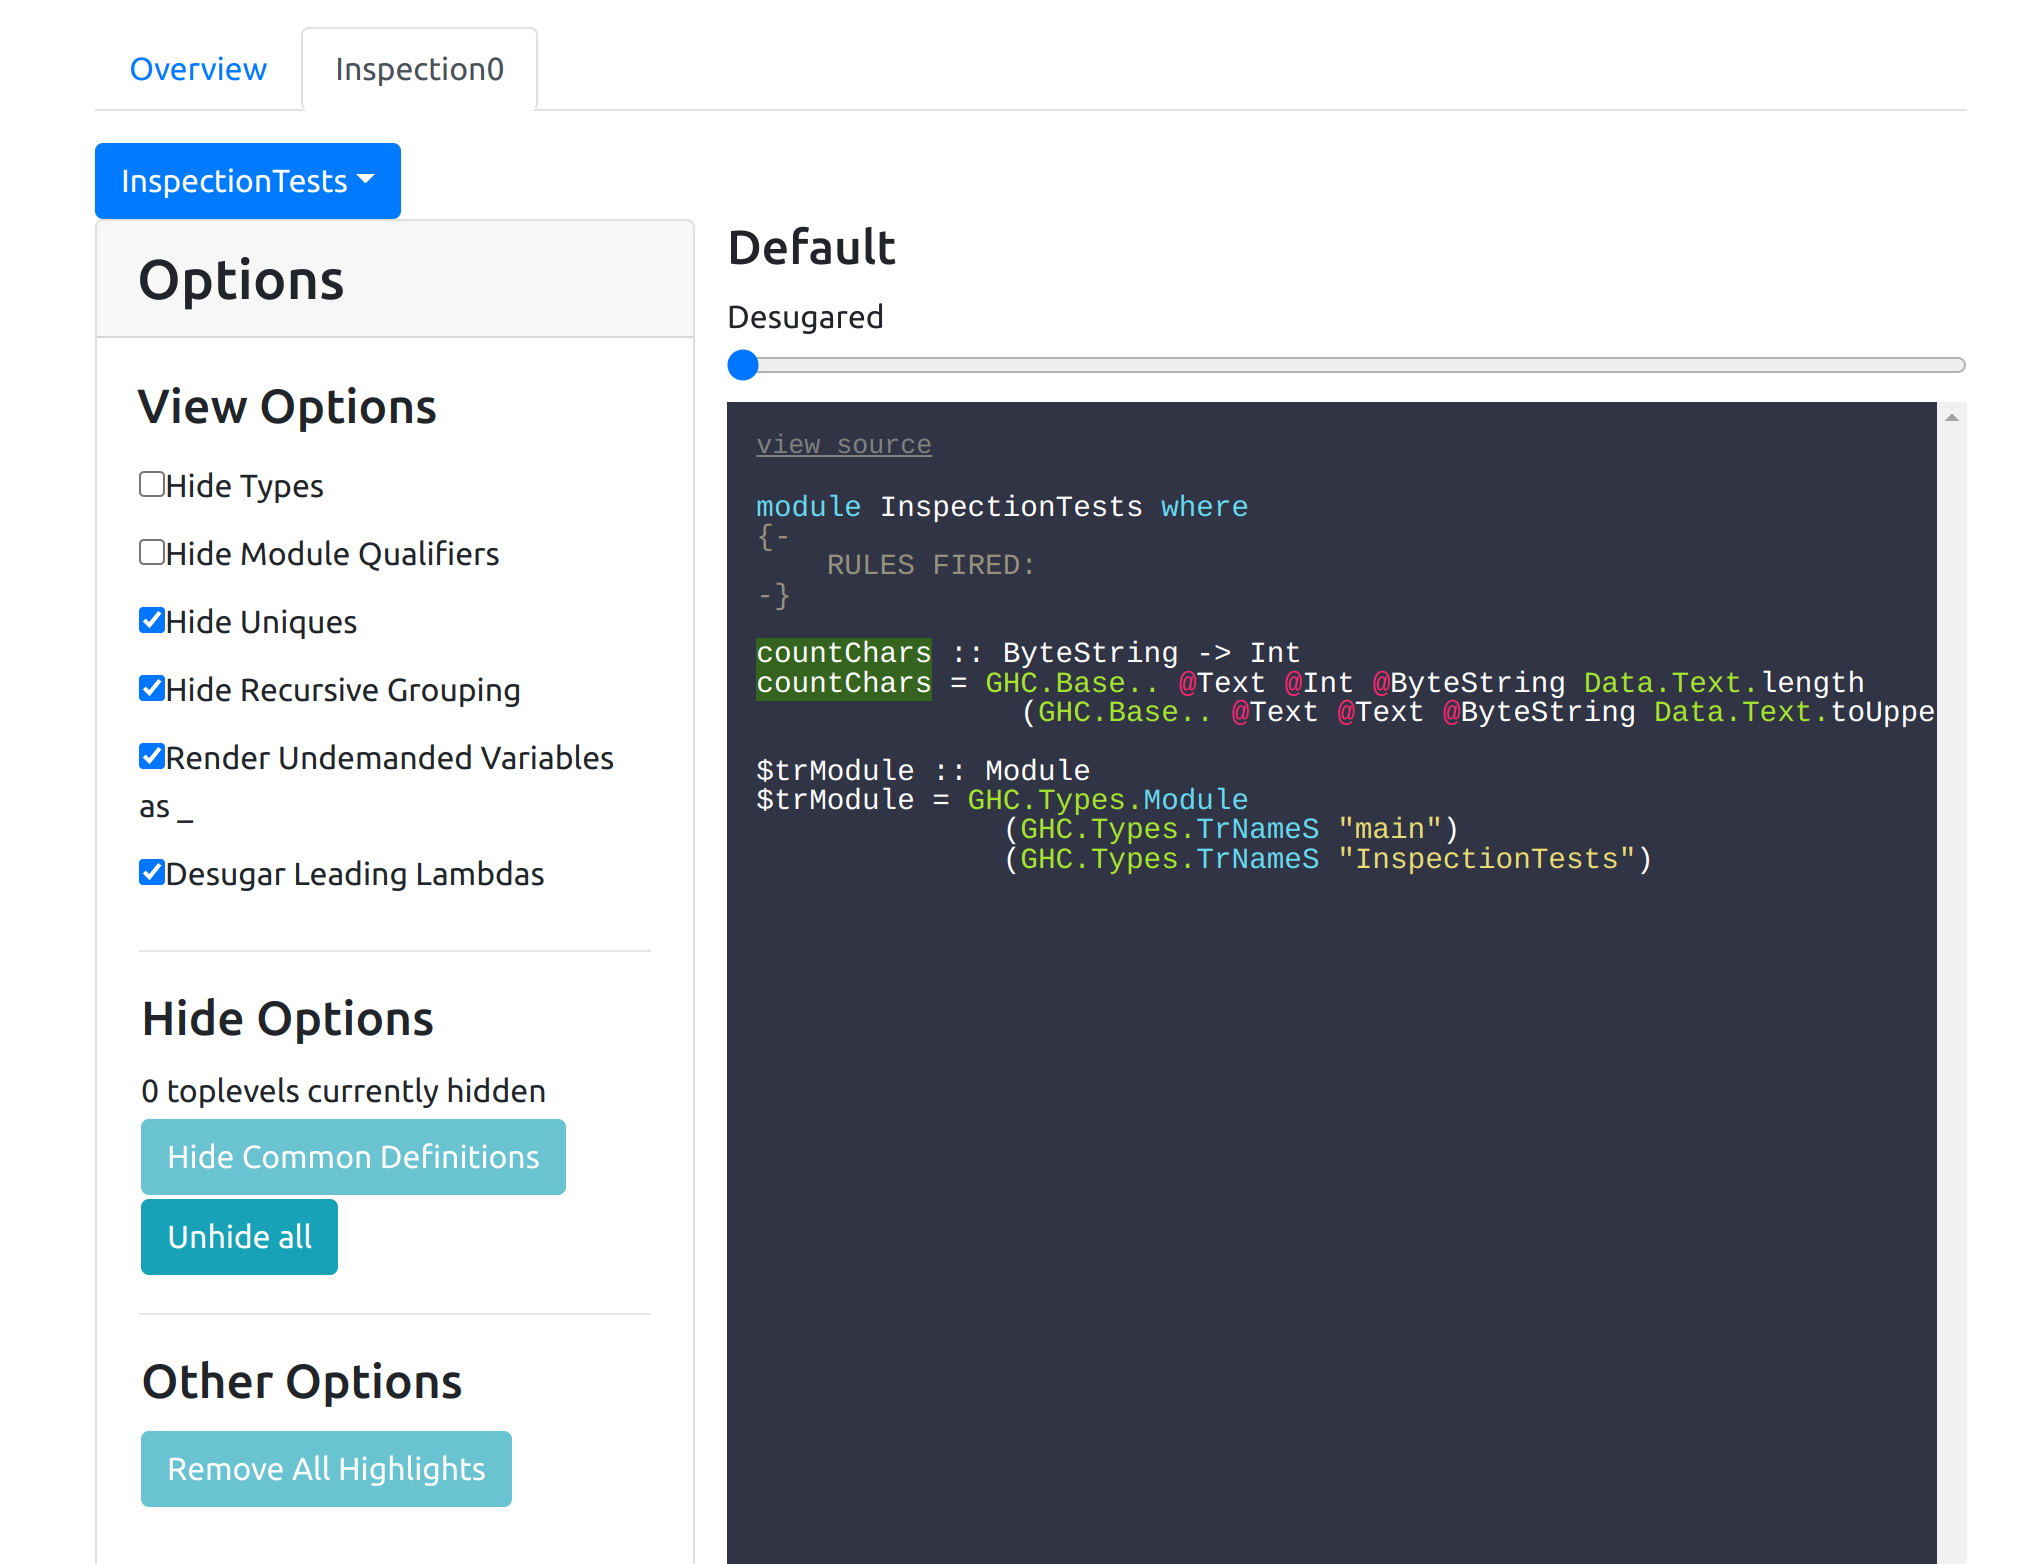
\includegraphics[width=0.8\textwidth]{figs/countchars_2.png}
\label{fig:countchars_2}
\end{figure}

On the left, are immediately presented with a number of viewing options. To the right we can see the rendered
Core, under influence of the view options. Above it a slider indicating that we are looking at the
Core in the desugared stage (so without any transformations yet applied). Scrolling this slider will reveal
the intermediate Core ASTs that were produced by the compiler. Whenever rewrite rules are fired they are included
as comments at the top of the module.

As you can see, the desugaring process has produced another top-level definition, namely \$\mono{trModule}. Since we
not care for anything but our \mono{countChars} function at this time, we can elect to filter out all other definitions,
including those that will be generated in the future: 

\begin{figure}[H]
\centering
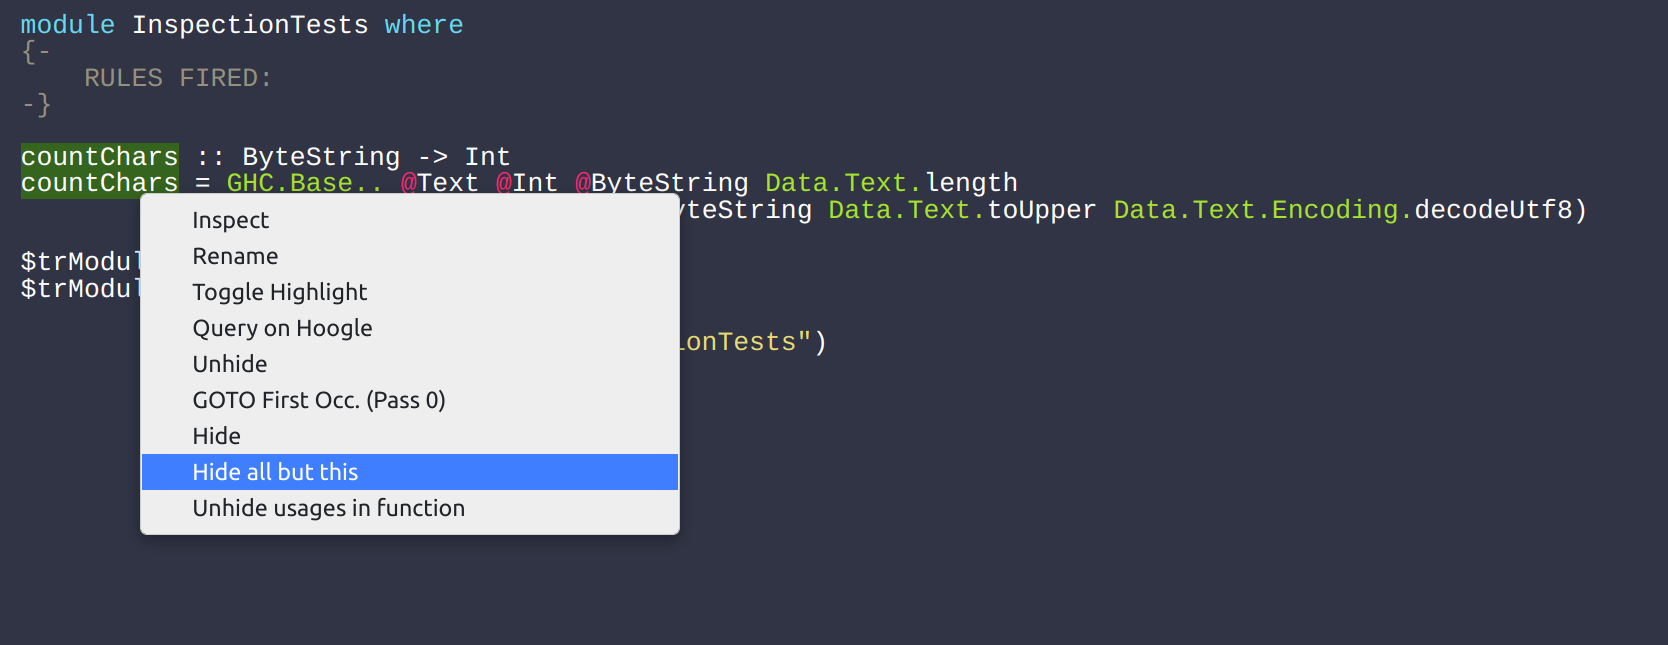
\includegraphics[width=0.8\textwidth]{figs/countchars_hideallbut.png}
\label{fig:countchars_3}
\end{figure}

If we then scroll all the way to the end, we get the same final Core AST as we saw in the error message. Granted,
we now have syntax highlighting and a slightly more readable representation, but it is still unwieldy. Using a basic string search we can find the needle in the haystack:

\begin{figure}[H]
\centering
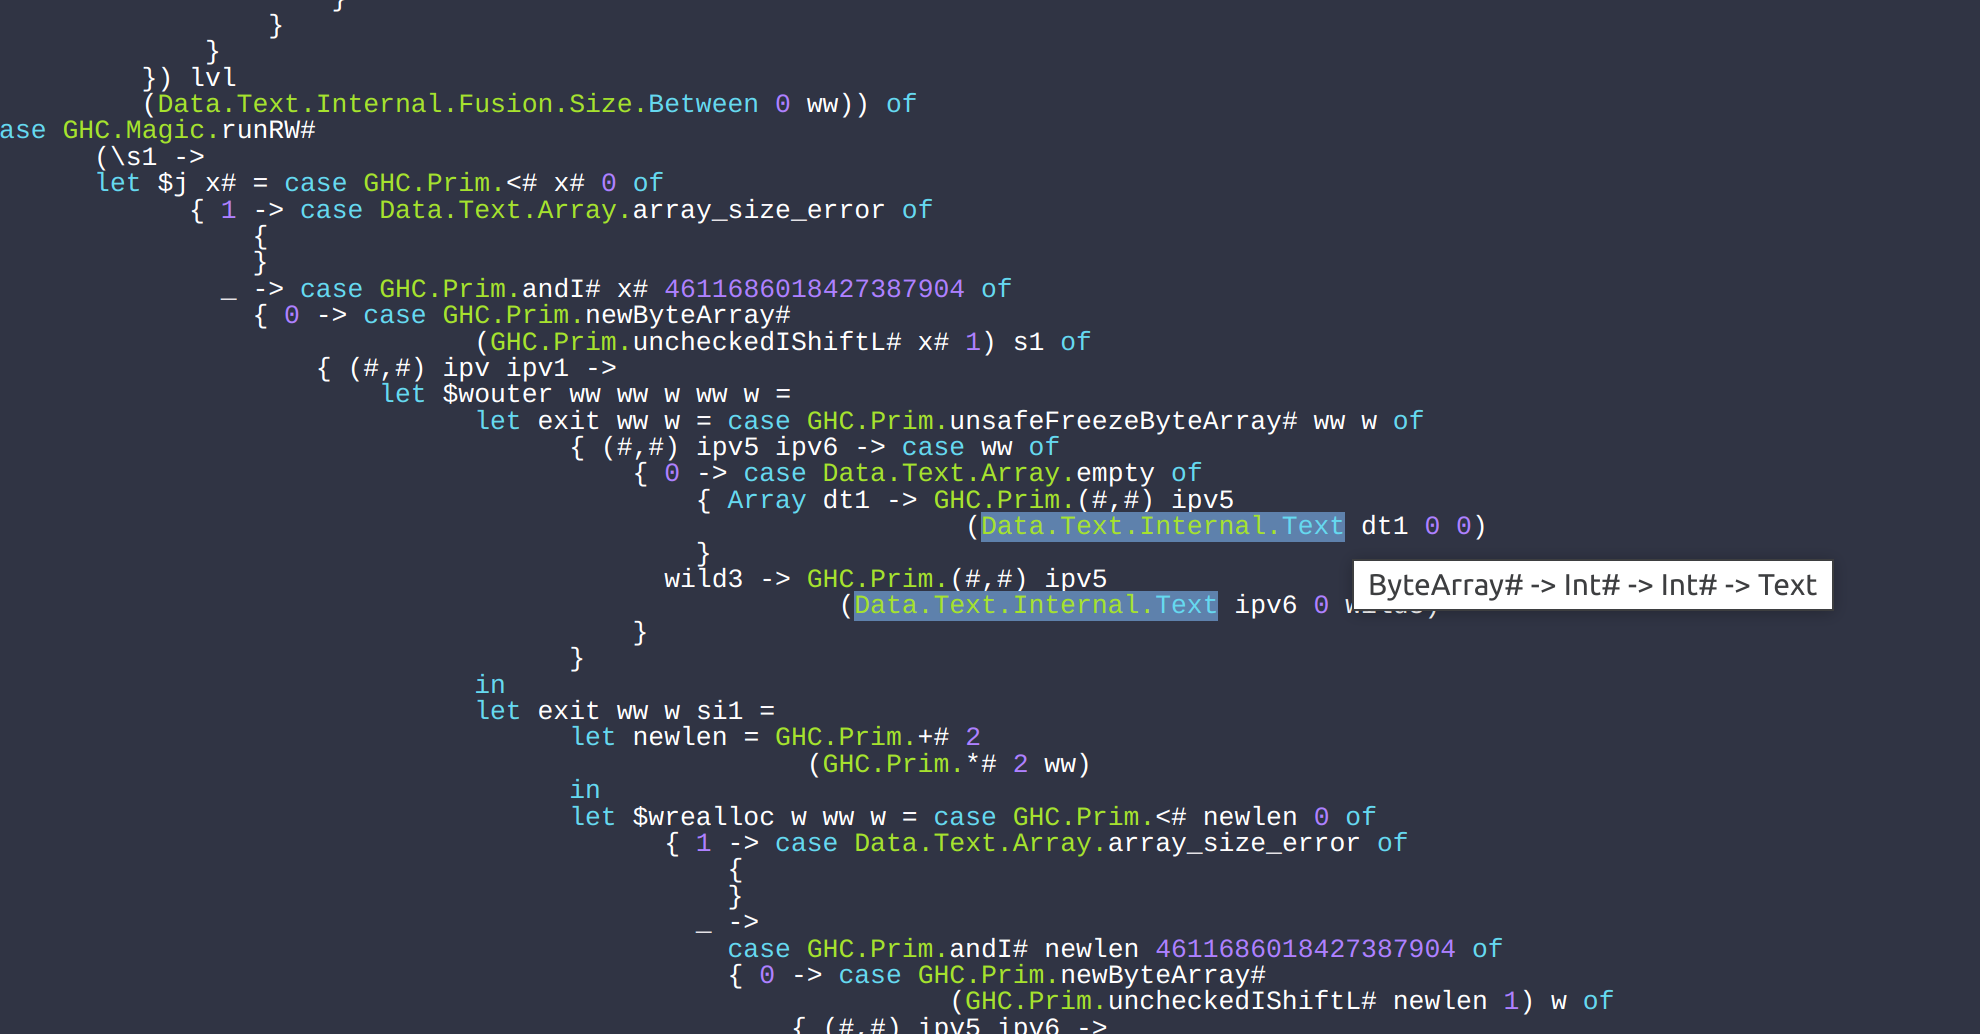
\includegraphics[width=0.8\textwidth]{figs/countchars_3.png}
\end{figure}

But we don't really care about finding the needle, but more so how it got it there.
Using the scroll bar we can go back in time to a moment before everything was inlined.
Specifically, we can go back to the first moment where no \mono{Text} constructor existed yet:

\begin{figure}[H]
\centering
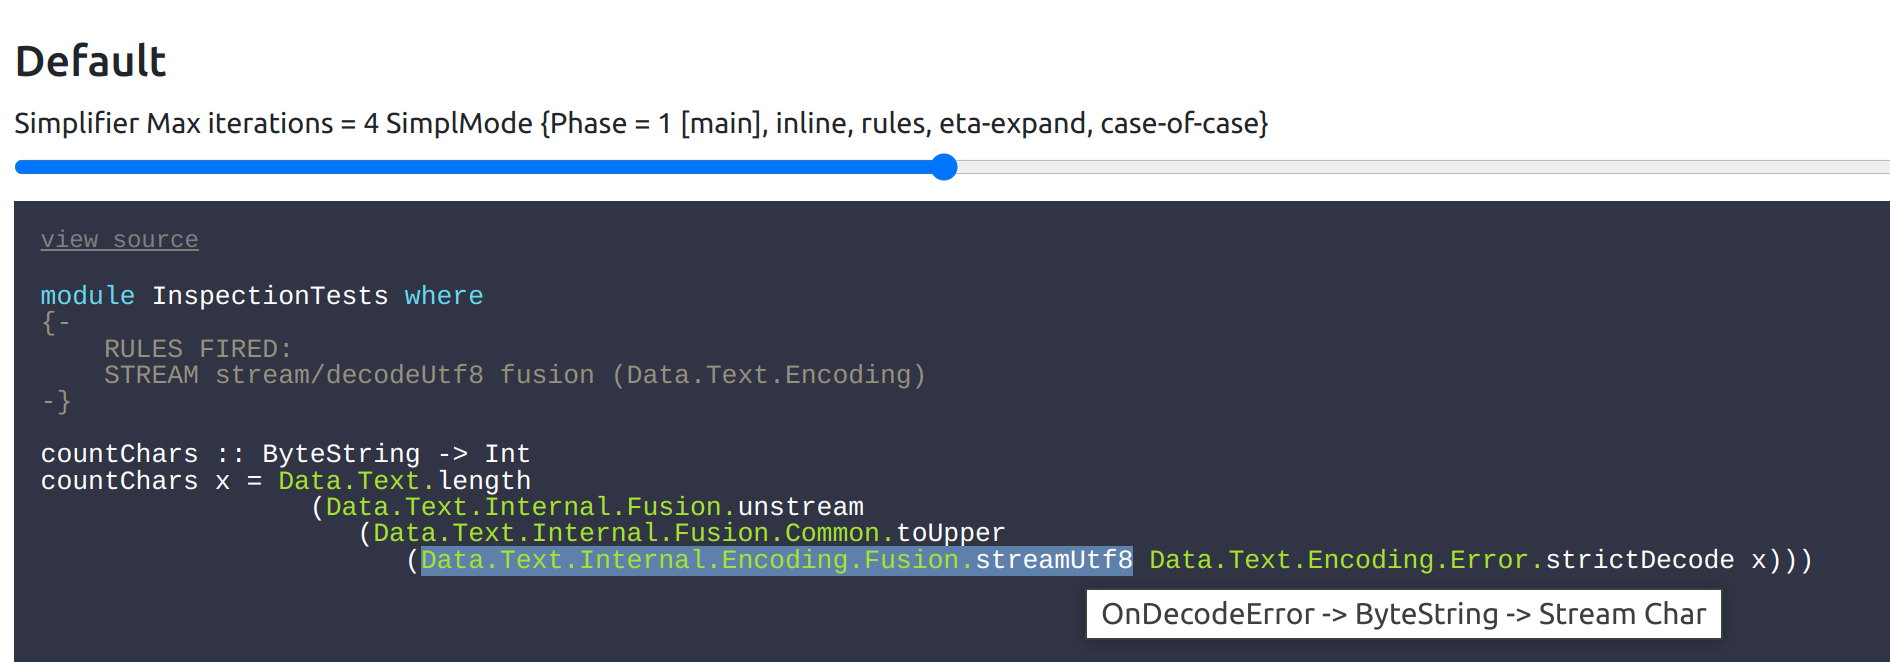
\includegraphics[width=0.8\textwidth]{figs/countchars_4.png}
\end{figure}

We find a far more manageable definition of \mono{countChars} that has partially been transformed to operate on streams (\mono{Stream Char}).
This is a concept to faciliate fusion based on the work of D. Couts et al. \cite{stream_fusion}, we will discuss its theory more
in depth in next section. For now, it is only important to realise that instead of embedding the
incoming \mono{ByteString} in a \mono{Text} value, we are converting to a \mono{Stream Char} first before \mono{unstream}
converts to an actual \mono{Text}. The argument that this is not necessary still holds because there conceivably exists a length
function for values of type \mono{Stream Char} as well. 

So we can conclude that the \mono{text}'s fusion machinery did not produce the optimal result because it is conceivable to find the
length of a stream directly using some alternative \mono{length :: Stream Char -> Int} function.

\paragraph{4. Back to the future}

Luckily, we were reliving someone else's experience, and we have the luxury of seeing how the situation unfolded.
So, what we can do is make another capture with a more recent version of the library, and compare the two:

\begin{figure}[H]
\centering
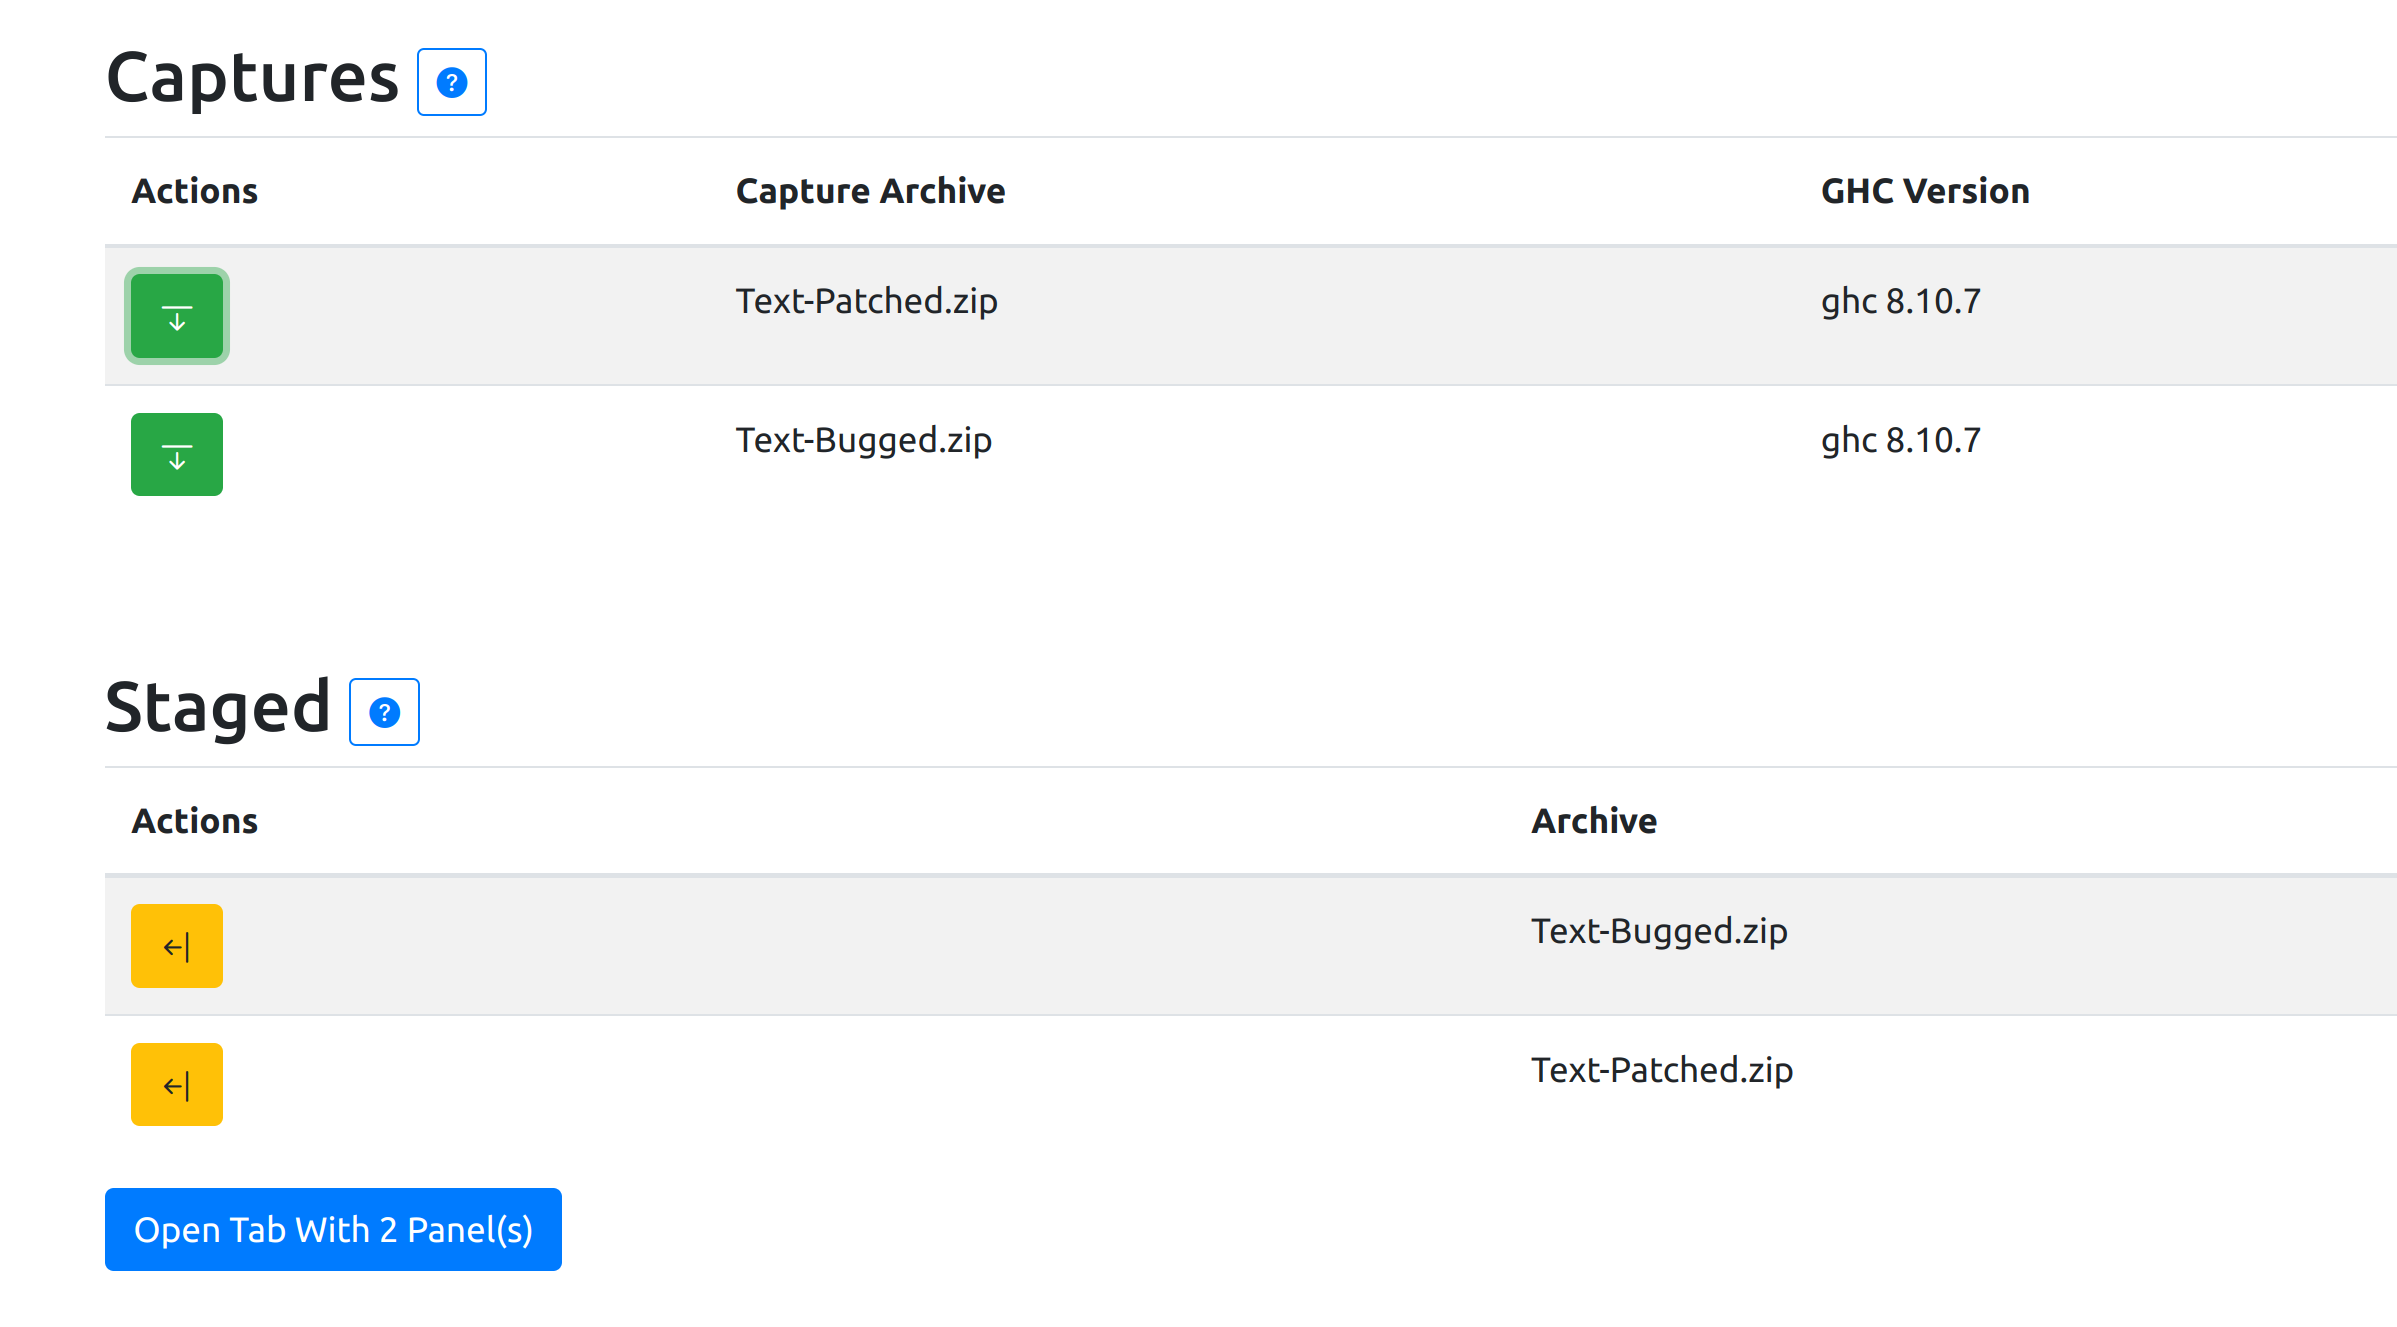
\includegraphics[width=0.8\textwidth]{figs/countchars_5.png}
\end{figure}

Because we now have more than 1 capture open at the same time we can use the \textit{Hide common definitions} feature to
find the first moment where the two captures converge. This happens to be at phase 1 of the simplifier pass:

\begin{figure}[H]
\centering
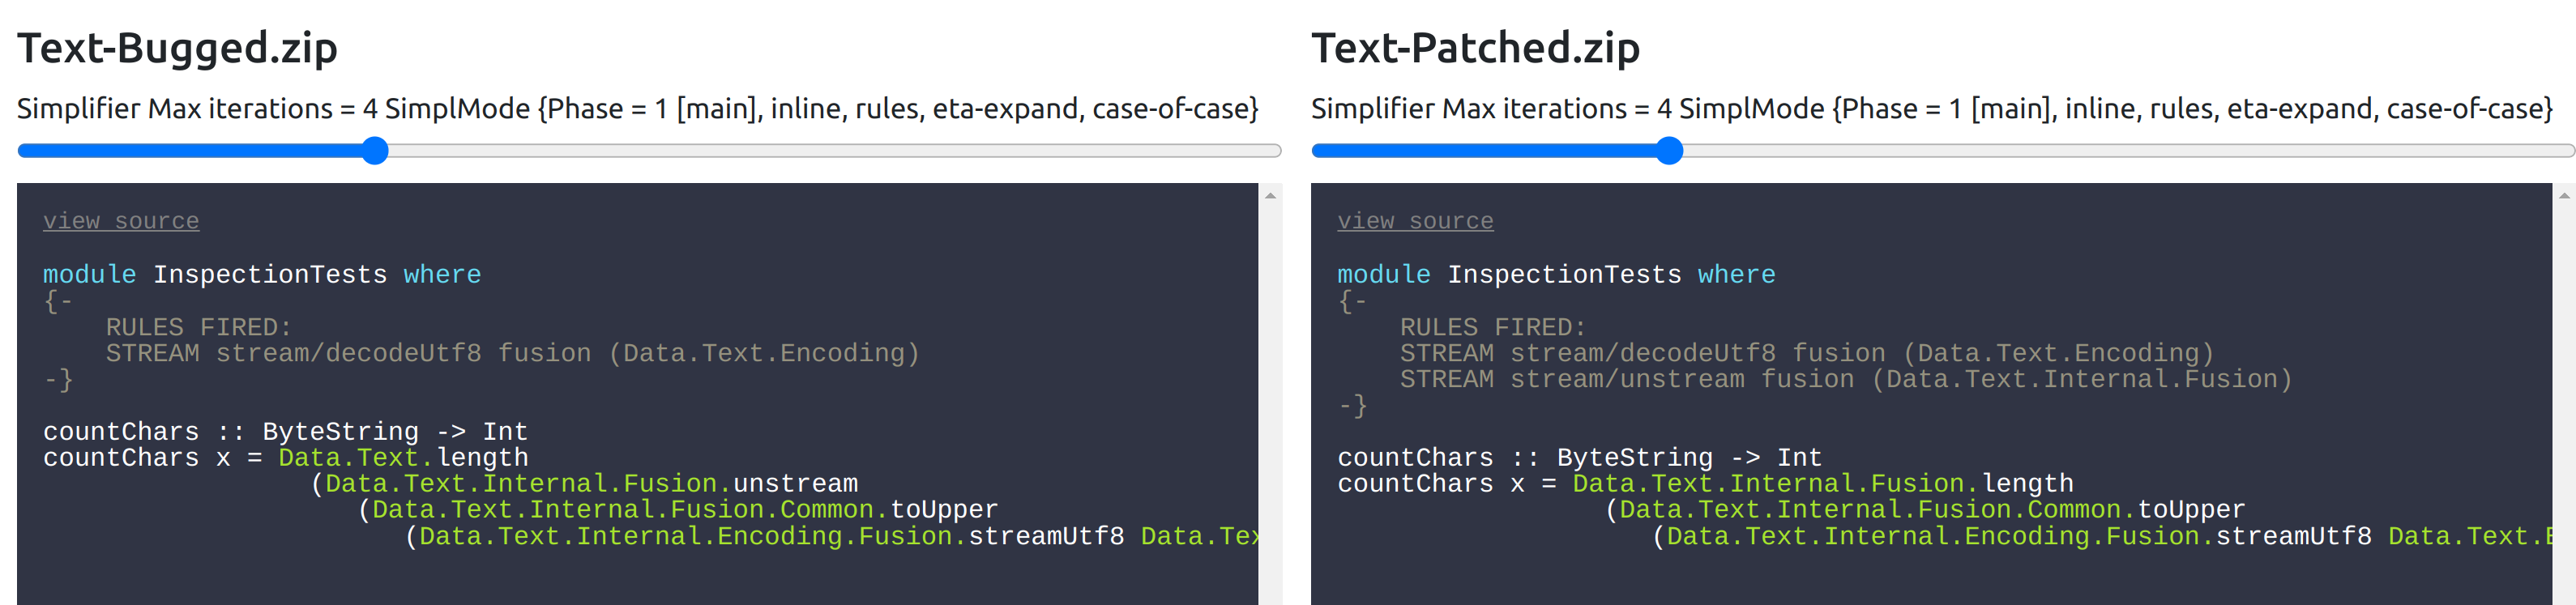
\includegraphics[width=0.9\textwidth]{figs/countchars_6.png}
\end{figure}

For clarity, let us extract the text from both panels and compare them:

\begin{listing}[H]
\begin{minted}[linenos,fontsize=\footnotesize]{haskell}
{-
    Text-Bugged.zip
    RULES FIRED:
    STREAM stream/decodeUtf8 fusion (Data.Text.Encoding)
-}

countChars :: ByteString -> Int
countChars x = Data.Text.length
                 (Data.Text.Internal.Fusion.unstream
                    (Data.Text.Internal.Fusion.Common.toUpper
                       (Data.Text.Internal.Encoding.Fusion.streamUtf8 Data.Text.Encoding.Error.strictDecode x)))

------------------------------------------------------------------
{-
    Text-Patched.zip
    RULES FIRED:
    STREAM stream/decodeUtf8 fusion (Data.Text.Encoding)
    STREAM stream/unstream fusion (Data.Text.Internal.Fusion)
-}

countChars :: ByteString -> Int
countChars x = Data.Text.Internal.Fusion.length
                 (Data.Text.Internal.Fusion.Common.toUpper
                    (Data.Text.Internal.Encoding.Fusion.streamUtf8 Data.Text.Encoding.Error.strictDecode x))
\end{minted}
\end{listing}

The most notable difference is the extra rewrite rule that was fired in the patched version (line 18).
Unfortunately, it is currently not possible to look up the definition of the rewrite rule in the tool itself, but
given that we know its name and originating module, we can find it in the source of \mono{text} without too much effort:

\begin{listing}[H]
\begin{minted}{haskell}
{-# RULES "STREAM stream/unstream fusion" forall s. stream (unstream s) = s #-}
\end{minted}
\end{listing}

From this we learn that at some point there was a stream/unstream pair to remove. Another difference is the module from which
the \mono{length} function is imported (\mono{Data.Text.Internal.Fusion.length} over \mono{Data.Text.length}). Like we predicted earlier,
the patched version uses a variant that operates directly on streams:

\begin{figure}[H]
\centering
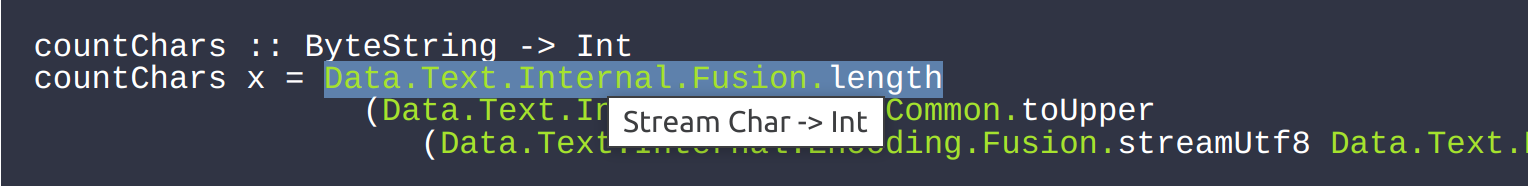
\includegraphics[width=0.8\textwidth]{figs/countchars_7.png}
\end{figure}

Given that in the previous in pass the captures were identical, and since no rewrite rule fired regarding \mono{length},
we can ascribe the difference to the inlining of \mono{length}. If we collect the definition of \mono{length} from both versions
of the text library we get:

\begin{listing}[H]
\begin{minted}{haskell}
-- Text-Bugged.zip
length :: Text -> Int
length t = S.length (stream t)
{-# INLINE [0] length #-}

-------------------------------------------

-- Text-Patched.zip
length :: Text -> Int
length t = S.length (stream t)
{-# INLINE [1] length #-}
\end{minted}
\end{listing}

The only difference is the phase annotation of the \mono{INLINE} pragma. The maintainers somehow decided that it was better
to inline \mono{length} one simplifier phase earlier (remember, phase 1 comes \textbf{before} phase 0). And they turned out to be right,
because inlining earlier uncovered the opportunity for the \textit{stream/unstream} rule to fire and remove 
the need to allocate an intermediate \mono{Text} value; Another exemplary manifestation of the Cascade Effect.

\paragraph{5. Epilogue: Brittleness of implicit fusion}
At or around the same time as Breitner. \cite{inspection_testing} identified the failed fusion case, Andrew Lelechenko had discovered
a problem involving the \mono{tail} function \cite{two_tails} under fusion. \mono{tail} just needs to drop the first character.
Despite needing to check whether to skip 1 or 2 bytes because of the UTF-16 encoding, this can be done in $O(1)$ time and memory.
Obviously this property should still hold when applying \mono{tail} twice in row. As it turns out, it does not. The following steps occur:

\begin{listing}[H]
\begin{minted}{haskell}
tail . tail
-- { inline to fusion variant }
unstream . S.tail . stream . unstream . S.tail . stream
-- { apply 'stream . unstream = id' }
unstream . S.tail . S.tail . stream
\end{minted}
\end{listing}

By constructing a stream we have become committed to traversing the entire structure where it was not needed at first,
yielding an $O(n)$ time and memory version after ``optimisation''. This is different from the situation in \mono{countChars},
where UTF-16 already dictated $O(n)$ runtime.

The ending to this story is quite simply that implicit fusion was disabled entirely \cite{two_tails} for similar functions.
Frequent \mono{text} contributor, Oleg Grenrus, remarked the following on the proposal to remove them:

\textit{``I think this is the right thing to do. Implicit fusion is unpredictable, and you explain, doesn't even work in simple cases.''}

Instead, users can now opt in by using the stream variant of such functions explicitly. This is a tragic example of how optimisation
can be unpredictable, and by extent, how people would favour predictability over automatic performance transformations that risk making the program slower.

\section{Lists vs Streams}

Besides short-cut fusion \cite{shortcut_fusion}, there has been research into other fusion frameworks. One such framework is \textit{stream fusion} \cite{stream_fusion}.
Amusingly, the GHC wiki page about optimisation still mentions that stream fusion will be the default in the future \cite{ghc_wiki_opt}. It is our understanding
that this is no longer the intention, as join points reveal fusion opportunities that are not possible with the stream fusion framework \cite{compiling_wo_continuations}.

Regardless, stream fusion makes for an interesting case study to explore its effects throughout the transformation pipeline. The original implementation accompanied by
the paper is still available an archive on Hackage and can reasonably easy be made to compile under modern GHC versions.

The big idea underlying stream fusion is actually not that different from the \textit{build/foldr} building blocks. Instead of creating an existentially typed
\mono{build} functions, an existentially typed datatype is used. Inside this datatype is a continuation function that produces the next element of the stream.
This next element can also be \mono{Skip} to indicate that the element should be dropped, or \mono{Done} to indicate that the stream is finished:

\begin{listing}[H]
\begin{minted}{haskell}
data Stream a = 
  forall s. Stream (s -> Step a s) s

data Step s a 
  = Yield a s 
  | Skip s 
  | Done
\end{minted}
\end{listing}

To gain a better intuition about how this type operates, it helps to consider the \mono{stream} and \mono{unstream} functions which facilitate back and forth
conversion to canonical lists:

\begin{listing}[H]
\begin{minted}[linenos]{haskell}
stream :: [a] -> Stream a
stream xs = Stream next xs
  -- the stream keeps track of the remaining list and peals of the
  -- head at each step
  where next []     = Done
        next (x:xs) = Yield x xs

unstream :: Stream a -> [a]
unstream (Stream next s) = go s
  -- effectively 'go' chains 'next' unto itself until a 'Done' is reached
  where go s = case next s of
          Done      -> []
          Skip s    -> go s
          Yield x s -> x : go s
\end{minted}
\end{listing}

One could describe a stream as a stateful generator function. In the case of \mono{stream} the state is a list, 
and in the case of \mono{unstream} the state is itself a stream. In the later case you could see the state as a continuation function.

Why would we want to introduce this rather complex type? The answer is that it allows us to write functions over streams that are
non-recursive and therefore be fused by already existing optimisations like inlining and the worker/wrapper transformation. But before
we get to that point, let us first redefine some common functions like \mono{map} and \mono{filter} in terms of streams:

\begin{listing}[H]
\begin{minted}[linenos]{haskell}
-- In both these functions the state is itself a stream
map_s :: (a -> b) -> Stream a -> Stream b
map_s f = Stream next
  -- replaces the 'next' function with one that applies 'f' to any 'Yield' and propagates itself
  where next (Stream next s) = case next s of
          Done       -> Done
          Skip s     -> Skip (Stream next s)
          Yield x s  -> Yield (f x) (Stream next s)

filter_s :: (a -> Bool) -> Stream a -> Stream a
filter_s p = Stream next'
  -- replaces the 'next' function witih one that maps 'Yield' to 'Skip' if 'p' holds and propagates itself
  where next' (Stream next s) = case next s of
          Done       -> Done
          Skip s     -> Skip (Stream next s)
          Yield x s  -> if p x then Yield x (Stream next s) else Skip (Stream next s)
\end{minted}
\end{listing}

These variants can be used to create drop-in replacements for the canonical built-in functions. It is important to realise that
these definitions are not subject to existing rewrite rule for the eponymous functions from \mono{Data.List}.

\begin{listing}[H]
\begin{minted}[linenos]{haskell}
map :: (a -> b) -> [a] -> [b]
map f = unstream . map_s f . stream

filter :: (a -> Bool) -> [a] -> [a]
filter p = unstream . filter_s p . stream
\end{minted}
\end{listing}

With our framework in place, we can now involve a recurring example, \mono{halves}:

\begin{listing}[H]
\begin{minted}[linenos]{haskell}
halves :: [Int] -> [Int]
halves = map (*2) . filter even
\end{minted}
\end{listing}

We already know how GHC's shortcut fusion will treat this function, so let us assume we are now using the stream fusion variants instead
and that we have convinced GHC to inline these definitions:

\begin{listing}[H]
\begin{minted}[linenos]{haskell}
halves :: [Int] -> [Int]
halves = unstream . map_s (*2) . stream . unstream . filter_s even . stream
\end{minted}
\end{listing}

This doesn't appear to be a good idea at all thus far, we are wasting a lot of work converting between streams and lists. However, there is a rather obvious
avenue for elimination given the equivalence \mono{stream . unstream = id}:

\begin{listing}[H]
\begin{minted}[linenos]{haskell}
{-# RULES "stream/unstream" forall s. stream (unstream s) = s #-}

--after firing
halves :: [Int] -> [Int]
halves = unstream . map_s (*2) . filter_s even . stream
\end{minted}
\end{listing}

Of course this only solved a problem we introduced ourselves in the first place, but this is the moment the big idea kicks in: 
because \mono{map_s} and \mono{filter_s} are not defined recursively, they are subject to inlining.
Using our tool we can observe what happens in practice during the transformation of \mono{halves}
without any further assumptions from the very start:

\begin{listing}[H]
\begin{minted}[linenos, fontsize=\footnotesize]{haskell}
--[0] Desugared
halves :: [Int] -> [Int]
halves xs = Data.List.Stream.map
              (
              let div_int = GHC.Real.div GHC.Real.$fIntegralInt
              in 
              let two = GHC.Types.I# 2
              in \v -> div_int v two)
              (Data.List.Stream.filter
                 (GHC.Real.even GHC.Real.$fIntegralInt) xs)
\end{minted}
\end{listing}

We have renamed the let bound variables to something descriptive.

\begin{listing}[H]
\begin{minted}[linenos, fontsize=\footnotesize]{haskell}
--[1] Simplifier [InitialPhase]
{-
    RULES FIRED:
    Class op div (BUILTIN)
    filter -> fusible (Data.List.Stream)
    map -> fusible (Data.List.Stream)
    STREAM stream/unstream fusion (Data.Stream)
-}

halves :: [Int] -> [Int]
halves xs = Data.Stream.unstream
              (Data.Stream.map
                 (
                 let two = GHC.Types.I# 2
                 in \v -> GHC.Real.$fIntegralInt_$cdiv v two)
                 (Data.Stream.filter
                    (GHC.Real.even GHC.Real.$fIntegralInt)
                    (Data.Stream.stream xs)))

\end{minted}
\end{listing}

\mono{map} and \mono{filter} have now been rewritten to their stream variants (by the two \textit {fusible} rules) and right after that
the complementing \mono{stream}/\mono{unstream} pair has been removed by the \textit {stream/unstream} rule.
The version we have now is effectively the same as our original hypothesis before we started exploring the real world situation.

\begin{listing}[H]
\begin{minted}[linenos, fontsize=\footnotesize]{haskell}
--[2] Specialise
$dReal :: Real Int
$dReal = GHC.Real.$p1Integral GHC.Real.$fIntegralInt

$dEq :: Ord Int
$dEq = GHC.Real.$p2Real $dReal

$dEq1 :: Eq Int
$dEq1 = GHC.Classes.$p1Ord $dEq

$dNum :: Num Int
$dNum = GHC.Real.$p1Real $dReal

$seven :: Int -> Bool
$seven n = GHC.Classes.== $dEq1
             (GHC.Real.rem GHC.Real.$fIntegralInt n
                (GHC.Num.fromInteger $dNum 2))
             (GHC.Num.fromInteger $dNum 0)

halves :: [Int] -> [Int]
halves xs = Data.Stream.unstream
              (Data.Stream.map
                 (
                 let two = GHC.Types.I# 2
                 in \v -> GHC.Real.$fIntegralInt_$cdiv v two)
                 (Data.Stream.filter
                    (GHC.Real.even GHC.Real.$fIntegralInt)
                    (Data.Stream.stream xs)))
\end{minted}
\end{listing}

The specialise phase has generated a couple -- currently unused -- auxiliary functions like \mono{seven} (`s' as in `specialised-even').
This definition will become relevant later as the resolver of finding a specific \mono{Num} instance.
We can expect to see this functions being used in the near future.

\begin{listing}[H]
\begin{minted}[linenos, fontsize=\footnotesize]{haskell}
-- [3] Float out

-- ... (omitted)

two :: Int
two = GHC.Types.I# 2

div2 :: Int -> Int
div2 v = GHC.Real.$fIntegralInt_$cdiv v two

even :: Int -> Bool
even = GHC.Real.even GHC.Real.$fIntegralInt

halves :: [Int] -> [Int]
halves xs = Data.Stream.unstream
              (Data.Stream.map div2
                 (Data.Stream.filter even
                    (Data.Stream.stream xs)))
\end{minted}
\end{listing}

The float out phase has, unsurprisingly, floated out some expressions to fresh top-level binds.

\begin{listing}[H]
\begin{minted}[linenos, fontsize=\footnotesize]{haskell}
-- [4] Simplifier [Phase=2]
{-
    RULES FIRED:
    Class op $p1Integral (BUILTIN)
    Class op $p2Real (BUILTIN)
    Class op $p1Ord (BUILTIN)
    Class op $p1Real (BUILTIN)
    Class op fromInteger (BUILTIN)
    Integer -> Int# (wrap) (BUILTIN)
    Class op fromInteger (BUILTIN)
    Integer -> Int# (wrap) (BUILTIN)
    Class op == (BUILTIN)
    Class op rem (BUILTIN)
    divInt# (BUILTIN)
    SPEC/Streaming even @Int (Streaming)
-}

zero :: Int
zero = GHC.Types.I# 0

$seven :: Int -> Bool
$seven n = case n of
  { I# ipv -> GHC.Classes.eqInt
                (GHC.Types.I#
                   (GHC.Prim.remInt# ipv 2)) lvl
  }

div2 :: Int -> Int
div2 v = case v of
  { I# ww1 -> GHC.Types.I#
                (GHC.Prim.uncheckedIShiftRA# ww1 1)
  }

halves :: [Int] -> [Int]
halves xs = Data.Stream.unstream
              (Data.Stream.map div2
                 (Data.Stream.filter $seven
                    (Data.Stream.stream xs)))
\end{minted}
\end{listing}

Simplified indeed, the specialised functions have been adopted and sometimes inlined.
However, any signs of fusion can not yet be found. Let's wind the clock forward another
transformation.

\begin{listing}[H]
\begin{minted}[linenos, fontsize=\footnotesize]{haskell}
--[5] Simplifier [Phase=1]
{-
    RULES FIRED:
    ==# (BUILTIN)
    tagToEnum# (BUILTIN)
    tagToEnum# (BUILTIN)
-}

$seven :: Int -> Bool
$seven n = case n of
  { I# ipv -> case GHC.Prim.remInt# ipv 2 of
      { 0 -> GHC.Types.True
        _ -> GHC.Types.False
      }
  }

div2 :: Int -> Int
div2 v = case v of
  { I# ww1 -> GHC.Types.I#
                (GHC.Prim.uncheckedIShiftRA# ww1 1)
  }

halves :: [Int] -> [Int]
halves xs = Data.Stream.unstream
              (Data.Stream.map div2
                 (Data.Stream.filter $seven
                    (Data.Stream.stream xs)))
\end{minted}
\end{listing}

Again still nothing exciting, only the \mono{zero} constant has been inlined.

\begin{listing}[H]
\begin{minted}[linenos, fontsize=\footnotesize]{haskell}
--[6] Simplifier [Phase=0]
{-
    RULES FIRED:
    Class op expose (BUILTIN)
    Class op expose (BUILTIN)
-}

$seven :: Int -> Bool
$seven n = case n of
  { I# ipv -> case GHC.Prim.remInt# ipv 2 of
      { 0 -> GHC.Types.True
        _ -> GHC.Types.False
      }
  }

halves :: [Int] -> [Int]
halves xs = 
  let unfold_unstream s1 = case s1 of
        { L ipv -> case ipv of
            { : x xs -> case x of
                { I# ipv -> case GHC.Prim.remInt# ipv 2 of
                    { 0 -> GHC.Types.:
                             (GHC.Types.I#
                                (GHC.Prim.uncheckedIShiftRA# ipv 1))
                             (unfold_unstream
                                (Data.Stream.L xs))
                      _ -> unfold_unstream
                             (Data.Stream.L xs)
                    }
                }
              [] -> GHC.Types.[]
            }
        }
  in unfold_unstream
       (Data.Stream.L xs)
\end{minted}
\end{listing}

Now something quite drastic has changed and it is not clear what exactly has happened. Let's first investigate
what the rewrite rule that just fired twice contributed to these changes. \mono{Class op {f}} implies that the 
function \mono{f} as part of some class constraint was specialised. If we scour the source we find the following
typeclass:

\begin{listing}[H]
\begin{minted}[linenos, fontsize=\footnotesize]{haskell}
class Unlifted a where

  -- | This expose function needs to be called in folds/loops that consume
  -- streams to expose the structure of the stream state to the simplifier
  -- In particular, to SpecConstr.
  --
  expose :: a -> b -> b
  expose = seq

  -- | This makes GHC's optimiser happier; it sometimes produces really bad
  -- code for single-method dictionaries
  --
  unlifted_dummy :: a
  unlifted_dummy = error "unlifted_dummy"
\end{minted}
\end{listing}

Supposedly this class is implemented for \mono{Stream a}, as those are terms that are affected, and indeed we find:

\begin{listing}[H]
\begin{minted}[linenos, fontsize=\footnotesize]{haskell}
instance Unlifted (Stream a) where
  expose (Stream next s0) s = seq next (seq s0 s)
  {-# INLINE expose #-}
\end{minted}
\end{listing}

From this we can speculate that this typeclass exists to ensure that expressions are evaluated to WHNF (by definition of \mono{seq}),
which is a requirement to ensure that other optimisations fire.

But we have not seen any callsite for \mono{expose} in the code, so apparently it appeared somehow \textbf{and} was specialised 
during this transformation. The most logical explanation for new function calls appearing is that they were the result of an inlining.
Our suspects are on the four stream functions:

\begin{itemize}
\item \mono{stream}
\item \mono{map}
\item \mono{filter}
\item \mono{unstream}
\end{itemize}

By inspecting each definition it turns out that of those suspects only \mono{unstream} contains calls to \mono{expose}:

\begin{listing}[H]
\begin{minted}[linenos, fontsize=\footnotesize]{haskell}
unstream :: Stream a -> [a]
unstream (Stream next s0) = unfold_unstream s0
  where
    unfold_unstream !s = case next s of
      Done       -> []
      Skip    s' -> expose s' $     unfold_unstream s'
      Yield x s' -> expose s' $ x : unfold_unstream s'
{-# INLINE [0] unstream #-}
\end{minted}
\end{listing}

Our expectations are further confirmed by the inline pragma which says to inline only at phase 0, which exactly what we think happened.
The same inline pragma is present on all of our other suspects as well, so we are looking a quadruple inlining event. The calls to \mono{seq}
are desugared as case expressions, as they are the primitive operation in Core that evaluates to WHNF.

Not all questions are answered however, as we don't know what the \mono{L} constructor does. Again, looking that up gives the following source:

\begin{listing}[H]
\begin{minted}[linenos, fontsize=\footnotesize]{haskell}
-- | Boxes for user's state. This is the gateway for user's types into unlifted
-- stream states. The L is always safe since it's lifted/lazy, exposing/seqing
-- it does nothing.
-- S is unlifted and so is only suitable for users states that we know we can
-- be strict in. This requires attention and auditing. 
--
data    L a = L a  -- lazy / lifted
newtype S a = S a  -- strict / unlifted
\end{minted}
\end{listing}

It seems that \mono{L} is just a box around a type that provides a barrier for WHNF evaluation. We can find it being used in the
definition of \mono{stream}:

\begin{listing}[H]
\begin{minted}[linenos, fontsize=\footnotesize]{haskell}
stream :: [a] -> Stream a
stream xs0 = Stream next (L xs0)
  where
    {-# INLINE next #-}
    next (L [])     = Done
    next (L (x:xs)) = Yield x (L xs)
    {-# INLINE [0] stream #-}
\end{minted}
\end{listing}

In essence, it just cancels the effect of \mono{seq}. But if we are careful then in some situation we might improve performance by using the
strict version \mono{S} instead. 

So that aside, have we achieved fusion? It takes some time to realise that, (1) through the use of \mono{expose} in the definition of \mono{unstream}, and (2)
by the direct use of the incoming \mono{next} function in the definition of the following next function, our resulting list has a head element that is defined
as the composition of \mono{next} function of \mono{map} and \mono{filter}. This is a very contrived way to say that we have indeed achieved fusion.

But we are still left with some noise, notably the wrapping/unwrapping of values in now redundant \mono{L} constructors. That description should invoke
a sense of familiarity, as the reader should know by know that an upcoming transformation is that of the \textit{worker/wrapper}!
If follow the rest of the pipeline in chronological order:

\begin{listing}[H]
\begin{minted}[linenos, fontsize=\footnotesize]{haskell}
-- [7] Float inwards
-- no changes

-- [8] Called arity analysis
-- no structural changes (IdInfos might be updated)

-- [9] Simplifier [Phase = Final]
-- no changes

-- [10] Demand analysis
-- no structural changes (IdInfos might be updated)

-- [11] Constructed Product Result analysis
-- no structural changes (IdInfos might be updated)

-- [12] Worker/wrapper binds
halves :: [Int] -> [Int]
halves xs = 
  let $wunfold_unstream ww = 
        let w = Data.Stream.L ww
        in 
        let s1 = w
        in case s1 of
        { L ipv -> case ipv of
            { : x xs -> case x of
                { I# ipv -> case GHC.Prim.remInt# ipv 2 of
                    { 0 -> GHC.Types.:
                             (GHC.Types.I#
                                (GHC.Prim.uncheckedIShiftRA# ipv 1))
                             (unfold_unstream
                                (Data.Stream.L xs))
                      _ -> unfold_unstream
                             (Data.Stream.L xs)
                    }
                }
              [] -> GHC.Types.[]
            }
        }
      unfold_unstream w = case w of
        { L ww -> $wunfold_unstream ww
        }
  in unfold_unstream
       (Data.Stream.L xs)
\end{minted}
\end{listing}

From the \mono{w} prefix in the name of \mono{wunfold_unstream} we can derive that this function was generated by the worker/wrapper transformation.
This specific piece of knowledge is not strictly necessary however since our tool can tell you for any function in which pass it was generated regardless
of name.

If you look through the let bindings, it becomes apparent that we wrap an element \mono{ww} in an \mono{L} constructor, and then always evaluate it to WHNF
in the case expression. This is a classic wasteful pattern that the simplifier is able to deal with:

\begin{listing}[H]
\begin{minted}[linenos, fontsize=\footnotesize]{haskell}
-- [13] Simplifier [Phase = Final]
halves :: [Int] -> [Int]
halves xs = 
  let $wunfold_unstream ww = case ww of
        { : x xs -> case x of
            { I# ipv -> case GHC.Prim.remInt# ipv 2 of
                { 0 -> GHC.Types.:
                         (GHC.Types.I#
                            (GHC.Prim.uncheckedIShiftRA# ipv 1))
                         ($wunfold_unstream xs)
                  _ -> $wunfold_unstream xs
                }
            }
          [] -> GHC.Types.[]
        }
  in $wunfold_unstream xs
\end{minted}
\end{listing}

With that final elision we have obtained a fully fused version of our \mono{map}/\mono{filter} composition with any auxiliary machinery like \mono{stream} and
\mono{unstream} being fused away. 

So what we have shown is that it is perfectly feasible to create and retrofit an alternative fusion system in vanilla Haskell. 
However, it is also clear that the process of implementating it goes beyond translating the theory verbatim. Namely, we have seen how \mono{Unlifted} class was necessary to ensure that
GHC correctly handles lazy and strict situation, including the need to put an extra unused function in the typeclass to avoid some unexpected GHC behavior.
All this tells us that the developers of the library have most certainly spent a large chunk of their time looking at Core printouts to identify these issues before
there were able to fix it like they did. 

Furthermore, it was with the help of our tool that we were able to explain -- without direct consultation and within a reasonable timeframe -- 
how stream fusion truly operates in a real world scenario. This means that our tool may support those trying to reproduce and verify existing research
involving Haskell and the GHC compiler.

\section{Erroneous program structure recovery in GHC fusion}
\label{section:results:unlines}

As part of our initial experiments to validate the tool, we decided to attempt to reproduce the shot-cut fusion of \mono{unlines} as presented
in its introductory the paper \cite{shortcut_fusion}. This serendipitously led to the discovery of an important performance bug in GHC.

\subsection{The problem described}
Consider the implementation of unlines given in the paper:

\begin{listing}[H]
\begin{minted}[linenos]{haskell}
unlines :: [String] -> String
unlines ls = concat (map (\l -> l ++ ['\n']) ls)
\end{minted}
\end{listing}

Using our tool, it can be observed to be optimised to the following Core:

\begin{listing}[H]
\begin{minted}[linenos]{haskell}
cr_chr :: Char
cr_chr = C# '\n'

cr :: [Char]
cr = : cr_chr []

go1 :: [[Char]] -> [Char]
go1 ds = case ds of
  { : y ys -> ++
                (++ y cr)
                (go1 ys)
    [] -> []
  }

unlines :: [String] -> String
unlines ls = go1 ls
\end{minted}
\end{listing}

This definition is problematic because every line is traversed once to append a newline character and then again to append it to the rest of the line
yielding an $O(n^2)$ runtime, while we already know that an $O(n)$ runtime is possible. To rule out any other factors we ran a benchmark on both
\mono{unlines} and \mono{Prelude.unlines} on the first 73 lines of lorem ipsum, confirming our suspicions.

\begin{listing}[H]
\begin{minted}{text}
benchmarking our_unlines
time                 127.9 μs   (125.0 μs .. 130.7 μs)
                     0.997 R²   (0.996 R² .. 0.998 R²)
mean                 126.6 μs   (124.6 μs .. 128.4 μs)
std dev              6.532 μs   (5.742 μs .. 7.504 μs)
variance introduced by outliers: 53% (severely inflated)

benchmarking prelude_unlines
time                 80.23 μs   (79.87 μs .. 80.53 μs)
                     1.000 R²   (0.999 R² .. 1.000 R²)
mean                 79.70 μs   (79.05 μs .. 80.13 μs)
std dev              1.858 μs   (1.088 μs .. 2.962 μs)
variance introduced by outliers: 20% (moderately inflated)
\end{minted}
\end{listing}

So it is clear that \mono{Prelude} has defined \mono{unlines} in a more efficient manner, but that does not take away the fact that any such
expression as our version of \mono{unlines} should reasonably be expected to fuse to something $O(n)$ (it was the example given the original paper after all \cite{shortcut_fusion}).

\subsection{Investigating the problem}

Our approach to investigating this issue is to scroll all the way back to the desugared stage and see if we can find a distinct reason why the program was not transformed 
to something more optimal. Given that the culprit is a secondary list traversal, it is safe to assume that it is indeed the fusion system, or at least an iteraction with it,
that is at the root of this problem. Therefore, we decide to analyze the problem by seeking meaningful differences between the results of the transformation and the steps
given in the paper. The tool reports that the following Core is desugared from the source:

\begin{listing}[H]
\begin{minted}[linenos]{haskell}
unlines :: [String] -> String
unlines ls = concat $fFoldable[]
               (map
                  (\l -> ++ l
                           (build
                              (\c n -> c
                                         (C# '\n') n))) ls)
\end{minted}
\end{listing}

Here we can observe that the list literal \mono{['\n']} is already represented as a list producer function, paving the way for future short-cut fusion
rules applications. After all we can hypothesize that in the near future \mono{map} and \mono{++} will be rewritten to their respective \textit{build/foldr} representation,
making the fusion rule applicable. After the first transformation, which is the also first pass of the simplifier (Gentle), we get the following:

\begin{listing}[H]
\begin{minted}[linenos]{haskell}
{-
    RULES FIRED:
    Class op foldr (BUILTIN)
    ++ (GHC.Base)
    augment/build (GHC.Base)
    map (GHC.Base)
    fold/build (GHC.Base)
-}

unlines :: [String] -> String
unlines ls = build
               (\c n -> foldr
                          (mapFB
                             (\x y -> foldr c y x)
                             (\l -> build
                                      (\c n -> foldr c
                                                 (c
                                                    (C# '\n') n) l))) n ls)
\end{minted}
\end{listing}

We can see how concat has been specialized and also rewritten, as well as \mono{++}. The result of \mono{map} however, is a bit more peculiar; contrary to what the paper
suggested at the time, we instead observe a call to some function \mono{mapFP}. We keep this observation in mind and continue on.
The first pass that makes any significant change is the float out pass, which floats bindings up to the highest level to expose potential optimisations like
common expression elimination:

\begin{listing}[H]
\begin{minted}[linenos]{haskell}
cr_chr :: Char
cr_chr = C# '\n'

append_cr :: [Char] -> [Char]
append_cr l = build
                (\c n -> foldr c
                           (c cr_chr n) l)

unlines :: [String] -> String
unlines ls = build
               (\c n -> foldr
                          (mapFB
                             (\x y -> foldr c y x) append_cr) n ls)
\end{minted}
\end{listing}

In essence, nothing has significantly changed, let us continue. Simplifier phase 2 comes and goes without modifying the code. Simplifier phase 1 reduces to:

\begin{listing}[H]
\begin{minted}[linenos]{haskell}
{-
    RULES FIRED:
    foldr/app (GHC.Base)
    foldr/app (GHC.Base)
-}

cr_chr :: Char
cr_chr = C# '\n'

append_cr :: [Char] -> [Char]
append_cr l = ++ l
                (: cr_chr [])

unlines :: [String] -> String
unlines ls = foldr
               (mapFB ++ append_cr) [] ls
\end{minted}
\end{listing}

The only way can again find fusible pairs now is if we inline mapFB. We can easily find its definition by
right-clicking the term and selecting the \textit{Query on Hoogle} option. From there we can quickly get the
source code:

\begin{listing}[H]
\begin{minted}[linenos]{haskell}
-- Note eta expanded
mapFB ::  (elt -> lst -> lst) -> (a -> elt) -> a -> lst -> lst
{-# INLINE [0] mapFB #-} -- See Note [Inline FB functions] in GHC.List
mapFB c f = \x ys -> c (f x) ys
\end{minted}
\end{listing}

It seems that we may yet have a chance, simplifier phase 0 is the next pass and the annotation on \mono{mapFB} specifically
requests that we only inline the function is phase 0. However, we find the following after phase 0:

\begin{listing}[H]
\begin{minted}[linenos]{haskell}
cr_chr :: Char
cr_chr = GHC.Types.C# '\n'

unlines :: [String] -> String
unlines ls = 
  let go1 ds = case ds of
        { : y ys -> GHC.Base.++
                      (GHC.Base.++ y
                         (GHC.Types.: cr_chr GHC.Types.[]))
                      (go1 ys)
          [] -> GHC.Types.[]
        }
  in go1 ls
\end{minted}
\end{listing}

The version is nearly identical to the final Core produced by the entire pipeline, minus the inconsequential top-level binding introduced for constructing the newline
singleton string. So have discovered what went wrong? Well, not directly, but we have seen something that differs from the paper, namely the \mono{mapFB} function.
We might have already seen its definition, but it is not entirely clear what it does. Luckily, GHC has well documented source code, and so we return to Hoogle to find
the following note near the definition of \mono{mapFB}:

\begin{listing}[H]
\begin{minted}[linenos]{text}
{- Note [The rules for map]
~~~~~~~~~~~~~~~~~~~~~~~~~~~
The rules for map work like this.

* Up to (but not including) phase 1, we use the "map" rule to
  rewrite all saturated applications of map with its build/fold
  form, hoping for fusion to happen.

  In phase 1 and 0, we switch off that rule, inline build, and
  switch on the "mapList" rule, which rewrites the foldr/mapFB
  thing back into plain map.

  It's important that these two rules aren't both active at once
  (along with build's unfolding) else we'd get an infinite loop
  in the rules.  Hence the activation control below.

* This same pattern is followed by many other functions:
  e.g. append, filter, iterate, repeat, etc. in GHC.List

  See also Note [Inline FB functions] in GHC.List

* The "mapFB" rule optimises compositions of map

* The "mapFB/id" rule gets rid of 'map id' calls.
  You might think that (mapFB c id) will turn into c simply
  when mapFB is inlined; but before that happens the "mapList"
  rule turns
     (foldr (mapFB (:) id) [] a
  back into
     map id
  Which is not very clever.

* Any similarity to the Functor laws for [] is expected.
-}

{-# RULES
"map"       [~1] forall f xs.   map f xs                = build (\c n -> foldr (mapFB c f) n xs)
"mapList"   [1]  forall f.      foldr (mapFB (:) f) []  = map f
"mapFB"     forall c f g.       mapFB (mapFB c f) g     = mapFB c (f.g)
"mapFB/id"  forall c.           mapFB c (\x -> x)       = c
  #-}
\end{minted}
\end{listing}

This documentation does not give us any insight yet into the role of the \mono{mapFB} function. Perhaps the note \mono{[Inline FB functions]} can provide
some more insight:

\begin{listing}[H]
\begin{minted}[linenos]{text}
Note [Inline FB functions]
~~~~~~~~~~~~~~~~~~~~~~~~~~

After fusion rules successfully fire, we are usually left with one or more calls
to list-producing functions abstracted over cons and nil. Here we call them
FB functions because their names usually end with 'FB'. It's a good idea to
inline FB functions because:

* They are higher-order functions and therefore benefits from inlining.

* When the final consumer is a left fold, inlining the FB functions is the only
  way to make arity expansion to happen. See Note [Left fold via right fold].

For this reason we mark all FB functions INLINE [0]. The [0] phase-specifier
ensures that calls to FB functions can be written back to the original form
when no fusion happens.

Without these inline pragmas, the loop in perf/should_run/T13001 won't be
allocation-free. Also see Trac #13001.
\end{minted}
\end{listing}

Here we find a plausible answer to why \mono{mapFB} exists: ``\textit{alls to FB functions can be written back to the original form
when no fusion happens}''. It is desirable to retain the structure of the original map if it is not fused away (we will go more in depth in \cref{section:results:unlines:conclusion}).
\mono{mapFB} enables does just that,
it exposes an initial opportunity to fuse but is reversible using the \textit{mapList} rule if no fusion happens. This rule also gives us a lot of
intuition how \mono{mapFB} operates. Namely, given the cons function and an empty generator is equivalent to canonical \mono{map}. 
Similarly, the rule \textit{map} gives us information about how \mono{map} is more generally related to \mono{mapFB}. At this point we should
also compare how this \mono{foldr} based implementation differs from the one given in the paper:

\begin{listing}[H]
\begin{minted}[linenos]{haskell}
-- The definition from the short-cut fusion paper
map f xs = build (\ c n -> foldr (\a b -> c (f a) b) n xs)

-- The definition from GHC.Base
map f xs = build (\c n -> foldr (mapFB c f) n xs)
\end{minted}
\end{listing}

It does not take much convincing to see that the two definitions are syntactically equivalent after inlining mapFB.
Remember however the pragma instructing the compiler to inline mapFB \textbf{only} from phase 0 onwards. This turns out to be too late
and it is in the previous iteration of the simplifier (phase 1) where we overlooked something. Namely, the \textit{foldr/app} rule fired
twice. A grep in the GHC code base reveals its definition:

\begin{listing}[H]
\begin{minted}[linenos]{text}
"foldr/app"     [1] forall ys. foldr (:) ys = \xs -> xs ++ ys
        -- Only activate this from phase 1, because that's
        -- when we disable the rule that expands (++) into foldr
\end{minted}
\end{listing}

This rule appears to reverse the expansion of \mono{++}. This is corroborated by the reasoning behind activiting it in phase 1, otherwise it
would form a circular rule with the expansion the and the simplifier would exhaust its iterations without finding a fixed point. However, because
the reconstruction fired \textbf{before} the inlining of \mono{mapFB}, we missed out on an important fusion opportunity.


\subsection{Fixing the problem}

To confirm our theory about \mono{mapFB} clouding the fusion process, we can patch GHC in the following crude manner:

\begin{itemize}
  \item Redefine \mono{map} directly as \mono{build (\ c n -> foldr (\a b -> c (f a) b) n xs)} and mark it always as inlinable.
  \item Remove the \textit{map} rule, to prevent it firing instead of inlining.
  \item Remove the rule \textit{mapList}, \textit{mapFB}, and \textit{mapFB/id}, they should never be applicable anymore and there functionality
        now handled by the short-cut fusion rule.
\end{itemize}

For completeness:

\begin{listing}[H]
\begin{minted}[linenos]{haskell}
{-# INLINE map #-}
-- GHC.Base

-- previously:
map :: (a -> b) -> [a] -> [b]
map [] = []
map (x:xs) = f x : map f xs

-- now:
{-# INLINE map #-}
map :: (a -> b) -> [a] -> [b]
map f xs = build (\c n -> foldr (\x r -> c (f x) r) n xs)
\end{minted}
\end{listing}

Note that because previously map was defined recursively it would never have been inlined. In the new situation we inform GHC that we are actually very keen to
inline this function. If we feed the same source code to this patched version of GHC again we observe the following steps:

\begin{listing}[H]
\begin{minted}[linenos]{haskell}
==================== Simplifier [Gentle] ====================
unlines
  = \ls ->
      build
        (\ c n ->
           foldr
             (\x r -> foldr c (c (C# '\n'#) r) x)
             n
             ls)
\end{minted}
\end{listing}

GHC took our wishes to heart and inlined \mono{map} right away.

\begin{listing}[H]
\begin{minted}[linenos]{haskell}
==================== Simplifier [Phase = 1] ====================
cr_char = C# '\n'#

unlines
  = \ls ->
      foldr (\x r -> x ++ (lvl : r)) [] ls
\end{minted}
\end{listing}

Already we seem to be in a better place because we see only one call to \mono{++}. 
But things become clearer when foldr is inlined in the next simplifier phase:

\begin{listing}[H]
\begin{minted}[linenos]{haskell}
==================== Simplifier [Phase = 0] ====================
cr_char = C# '\n'

unlines
  = \ls ->
      let go ds =
          case ds of
            []      -> []
            y:ys -> y ++ (lvl : (go ys))
      in
      go ls
\end{minted}
\end{listing}

Although we still have a call to \mono{++} its left-hand side does not grow at each recursive iteration anymore. Furthermore, the other call to \mono{++} is
now correctly replaced by a much cheaper \textbf{prepend} action to the recursive call instead.
If run the same benchmark we observe that indeed our program is assembled to something significantly more efficient:

\begin{listing}[H]
\begin{minted}[]{text}
benchmarking my_unlines
time                 64.80 μs   (62.43 μs .. 66.47 μs)
                     0.996 R²   (0.995 R² .. 0.997 R²)
mean                 62.43 μs   (61.68 μs .. 63.40 μs)
std dev              2.779 μs   (2.062 μs .. 3.346 μs)
variance introduced by outliers: 48% (moderately inflated)

benchmarking prelude_unlines
time                 75.36 μs   (74.74 μs .. 75.80 μs)
                     1.000 R²   (1.000 R² .. 1.000 R²)
mean                 73.98 μs   (73.69 μs .. 74.35 μs)
std dev              1.102 μs   (886.1 ns .. 1.300 μs)
\end{minted}
\end{listing}

In fact, it seems we have managed to beat the performance of the prelude implementation by a small but real margin.

\subsection{It's more complicated}
\label{section:results:unlines:conclusion}

Seemingly we have solved the problem by returning to the original theory of the paper. But obviously the GHC developers did not simply
incorrectly implement the material. Functions like \mono{mapFB} do have a place. We already saw a hint of this in note from the source
code. To repeat:

\begin{listing}[H]
\begin{minted}[]{text}
...ensures that calls to FB functions can be written back to the original form when no fusion happens.
\end{minted}
\end{listing}

\mono{mapFB} provides gives us a tag that there used to be a call to \mono{map} here. If in the end we did not manage to fuse,
or if a \mono{mapFB} is left over after the \textit{mapFB} rules has combined consecutive instances, we can reconstruct the original
call to \mono{map}. This has two important befinits: First of all, it allows a more recognizable form of compiled Core that more closely
resembles the original source code. Secondly and arguably more importantly, we save on code size by reusing the map function by not
rewriting each list operation to a local, recursive \mono{go}.

Let us find a concrete example by comparing our patched version of GHC with the original one when compiling the very simple function:

\begin{listing}[H]
\begin{minted}[linenos]{haskell}
addTwo :: [Int] -> [Int]
addTwo = map (+1) . map (+1)
\end{minted}
\end{listing}

The Core produced looks this:

\begin{listing}[H]
\begin{minted}[linenos]{haskell}
-- Core from canonical GHC (total of 11 terms)
addTwo1 :: Int -> Int
addTwo1 x -> x+2

addTwo :: [Int] -> [Int]
addTwo xs -> map addTwo1 xs

-- Core from our patch (total of 23 terms)
addTwo :: [Int] -> [Int]
addTwo ds = case ds of
              [] -> []
              y : ys -> let xs = addTwo ys in x = y+2
                        in x:xs
\end{minted}
\end{listing}

This increased number of terms is a significant regression in compiled code size. 
However, we should not expect performance characteristics of the assembled code to differ much at all,
as they essentially describe the same computation.
We verify this by running a benchmark for \mono{addTwo [0..10000]}:

\begin{listing}[H]
\begin{minted}[]{text}
benchmarking addTwo_baseline
time                 79.70 μs   (79.61 μs .. 79.80 μs)
                     1.000 R²   (1.000 R² .. 1.000 R²)
mean                 79.71 μs   (79.67 μs .. 79.78 μs)
std dev              181.6 ns   (100.2 ns .. 336.0 ns)


benchmarking addTwo_patched
time                 79.17 μs   (78.80 μs .. 79.52 μs)
                     1.000 R²   (1.000 R² .. 1.000 R²)
mean                 79.74 μs   (79.40 μs .. 80.10 μs)
std dev              1.181 μs   (981.2 ns .. 1.436 μs)
\end{minted}
\end{listing}

Despite the regression in compiled code size, the argument could be made this trade off is worth it if in fact we can optimize more programs.
It should also be mentioned that our patch is very crude and does not take into account the subtle
interations with other existing rewrite rules; It is merelyl a confirmation of the problem.
It might be possible to find a more nuanced solution that still uses \mono{mapFB} but ensures it inlines
in time when it can be fused, but is still rewritten to \mono{map} otherwise.
Finding the ideal solution is not entirely trivial and an excellent topic for future work.

We have opened issue \href{https://gitlab.haskell.org/ghc/ghc/-/issues/22361}{\#22361} on the GHC bug tracker -- 
as well as a merge request with the proposed changes therein -- to spark a public conversation and collect telemetry on the impact of the change.
It should be noted that comments by both Sebastian Graf and Simon Peyton Jones were instrumental in helping us fully understand the problem and
the potential solution.

\section{Comparisons with existing approaches}

As we will discuss in detail in \cref{section:discussion:review}, we were unable to use the tool when working with unreleased
versions of GHC, something we had to do repeatedly during \cref{section:results:unlines}. As a silver lining, this presented
an excellent opportunity to compare the tool with the canonical existing approach: GHC flags.

An important milestone for us that when using \mono{-dsuppress-all}, the readability of the Core expressions is still not on par
with our tool. For clarity, we have cleaned manually edited the output of GHC to remove any irrelevant information. The original 
compiled Core definition of \mono{unlines} looked like this:

\begin{listing}[H]
\begin{minted}[linenos,fontsize=\footnotesize]{text}
-- RHS size: {terms: 2, types: 0, coercions: 0, joins: 0/0}
lvl_rVO :: GHC.Types.Char
[GblId, Unf=OtherCon []]
lvl_rVO = GHC.Types.C# '\n'#

-- RHS size: {terms: 3, types: 2, coercions: 0, joins: 0/0}
lvl1_rYZ :: [GHC.Types.Char]
[GblId, Unf=OtherCon []]
lvl1_rYZ
  = GHC.Types.:
      @GHC.Types.Char lvl_rVO (GHC.Types.[] @GHC.Types.Char)

Rec {
-- RHS size: {terms: 17, types: 18, coercions: 0, joins: 0/1}
Unlines.unlines_go1 [Occ=LoopBreaker]
  :: [[GHC.Types.Char]] -> [GHC.Types.Char]
[GblId, Arity=1, Str=<1L>, Unf=OtherCon []]
Unlines.unlines_go1
  = \ (ds_s11T [Occ=Once1!] :: [[GHC.Types.Char]]) ->
      case ds_s11T of {
        [] -> GHC.Types.[] @GHC.Types.Char;
        : y_s11V [Occ=Once1] ys_s11W [Occ=Once1] ->
          let {
            sat_s11Y [Occ=Once1, Dmd=ML] :: [GHC.Types.Char]
            [LclId]
            sat_s11Y = Unlines.unlines_go1 ys_s11W } in
          case GHC.Base.++ @GHC.Types.Char y_s11V lvl1_rYZ
          of sat_s11X [Occ=Once1]
          { __DEFAULT ->
          GHC.Base.++ @GHC.Types.Char sat_s11X sat_s11Y
          }
      }
end Rec }

-- RHS size: {terms: 3, types: 2, coercions: 0, joins: 0/0}
Unlines.unlines :: [GHC.Base.String] -> GHC.Base.String
[GblId, Arity=1, Str=<1L>, Unf=OtherCon []]
Unlines.unlines
  = \ (ls_s11Z [Occ=Once1] :: [GHC.Base.String]) ->
      Unlines.unlines_go1 ls_s11Z
\end{minted}
\end{listing}

As opposed to what the tool produces without any further manual effort such as renaming variables:

\begin{listing}[H]
\begin{minted}[linenos]{haskell}
lvl :: Char
lvl = C# '\n'

lvl :: [Char]
lvl = : lvl []

go1 :: [[Char]] -> [Char]
go1 ds = case ds of
  { : y ys -> ++
                (++ y lvl)
                (go1 ys)
    [] -> []
  }

unlines :: [String] -> String
unlines ls = go1 ls
\end{minted}
\end{listing}

We believe it goes without saying that our representation is faster to read and comprehend. Of course this is not entirely
fair because the GHC output contains for information that just happens to be uninteresting during many of our experiments.
That said, this information is still available upon request by double-clicking on any term to reveal all the embedded information:

\begin{figure}[H]
\centering
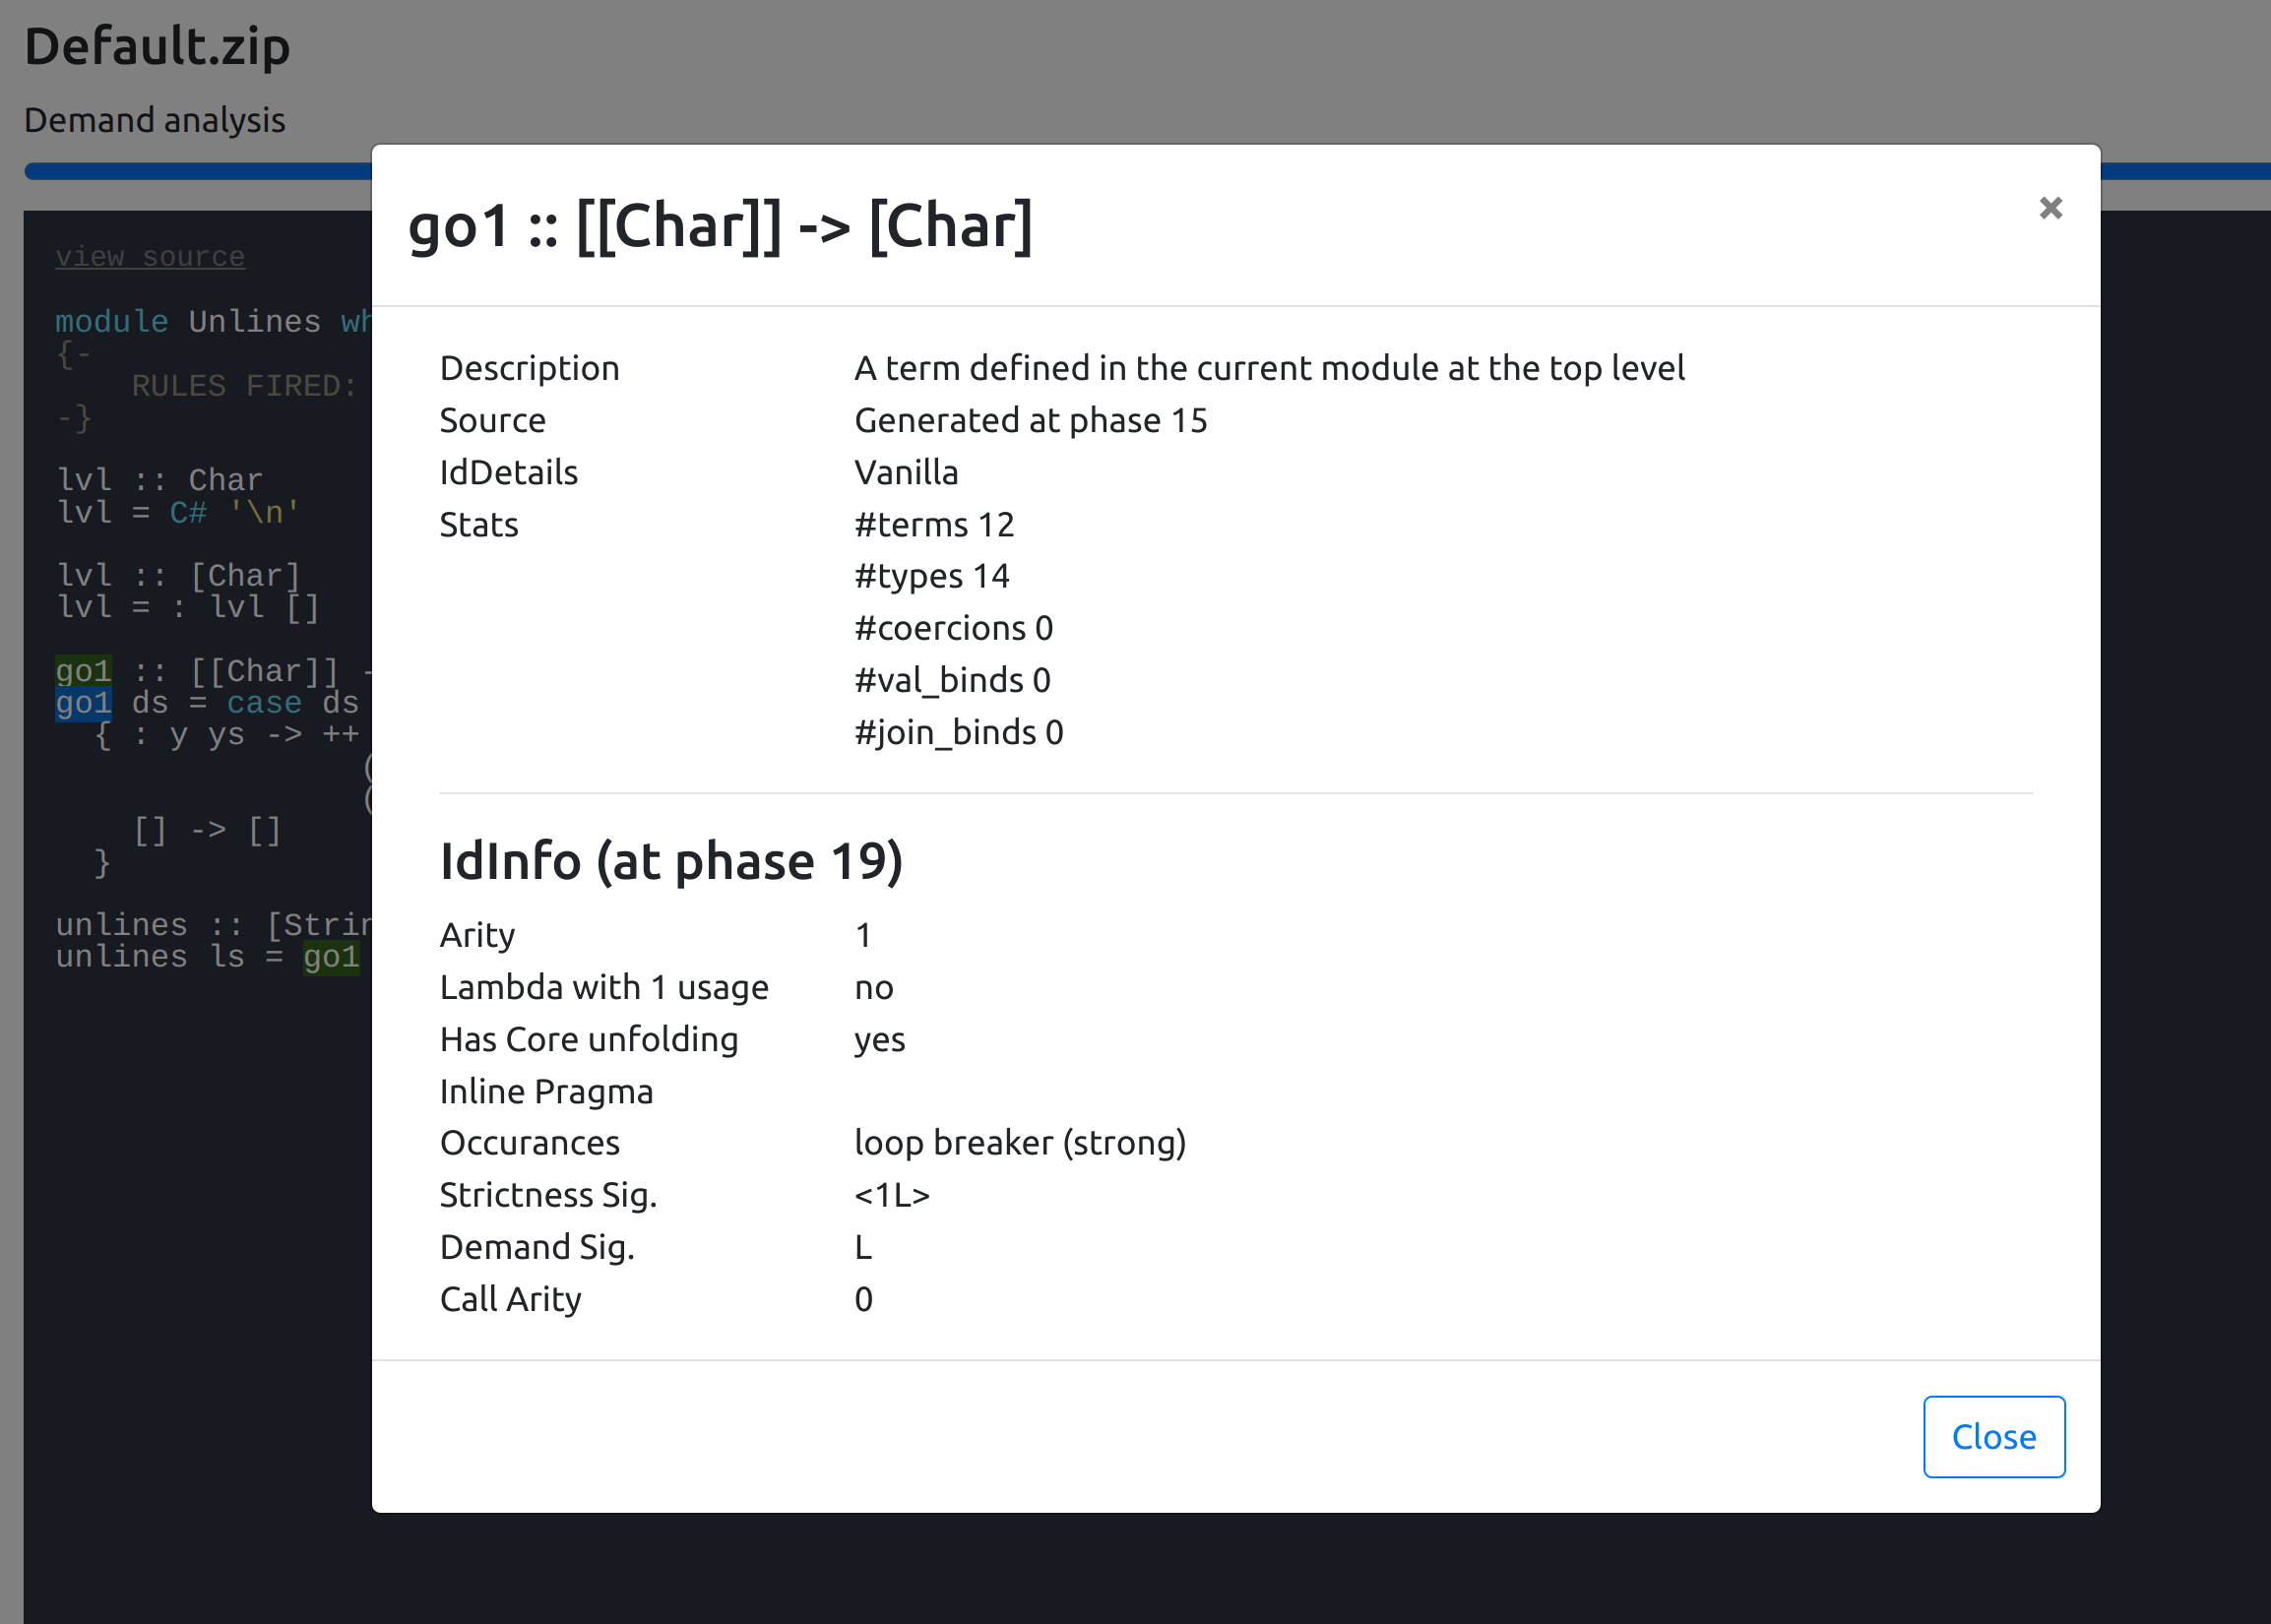
\includegraphics[width=0.8\textwidth]{figs/var_popup.png}
\caption{The popup that appears when double-clicking on a variable. It displays all available information embedded in the Core AST for that term.}
\label{fig:var-popup}
\end{figure}

This means that our tool is does not necessarily compromise on available information, but merely utilizes an interactive environment
to present the information less crudely. Clearly we were able to retrieve all the information needed from GHC, but our experience was
somewhat painful. By writing GHC's output to a file we could use features of most text editors like a string search to scroll through
the output of each pass. However, because of auxiliary definitions in the Core, the name of the current pass was usually not visible on
screen without having to scroll up. More importantly, which rewrite rules fired was also tough to attribute to a specific pass without
having to double-check regularly. In short, interpreting the textual output was more laborious and error prone that our newly developed
alternative.

In short, we find that our tool is much more pleasurable and productive experience over using GHC's compiler output, but this is of
course merely a subjective account. We hope that through our vision more people will agree that an improvement is possible and 
further debate ensues about how our existing solutions can be improved upon or inspire something better altogether.


